\documentclass[10pt]{article}

\usepackage[preprint]{arxiv_preprint}
% Float placement for the two-column layout.
\renewcommand{\topfraction}{0.9}          % single-column float may fill 90% of a column top
\renewcommand{\bottomfraction}{0.5}
\renewcommand{\textfraction}{0.07}
\renewcommand{\floatpagefraction}{0.6}    % single-column float page may be 60% full
\renewcommand{\dbltopfraction}{0.9}       % figure*/table* may fill 90% of a page top (default 0.7)
\renewcommand{\dblfloatpagefraction}{0.6} % figure*/table* float page may be 60% full (default 0.5)
\setcounter{topnumber}{3}
\setcounter{dbltopnumber}{3}              % up to 3 wide floats at the top of a page (default 2)
\setcounter{totalnumber}{5}
% Pack illustration-only pages from the top instead of stretching gaps between maps.
\makeatletter
\setlength{\@fptop}{0pt}
\setlength{\@fpsep}{6pt}
\setlength{\@fpbot}{0pt plus 1fil}
\setlength{\@dblfptop}{0pt}
\setlength{\@dblfpsep}{6pt}
\setlength{\@dblfpbot}{0pt plus 1fil}
\makeatother
\usepackage[utf8]{inputenc}
\usepackage[T1]{fontenc}
\usepackage{courier}
\usepackage{amsmath,amssymb,amsfonts}
% Mathematical Unicode symbols used in the included sections (pdfLaTeX).
\DeclareUnicodeCharacter{00D7}{\ensuremath{\times}}
\DeclareUnicodeCharacter{00F7}{\ensuremath{\div}}
\DeclareUnicodeCharacter{03C1}{\ensuremath{\rho}}
\DeclareUnicodeCharacter{2192}{\ensuremath{\rightarrow}}
\DeclareUnicodeCharacter{2212}{\ensuremath{-}}
\DeclareUnicodeCharacter{2264}{\ensuremath{\leq}}
\DeclareUnicodeCharacter{2265}{\ensuremath{\geq}}
\usepackage{booktabs}
\usepackage{longtable}
\usepackage{calc}
\usepackage{enumitem}
\usepackage{graphicx}
\usepackage{hyperref}
\usepackage{url}
\usepackage{microtype}
\usepackage{xcolor}
\usepackage{array}
\usepackage{tabularx}
\usepackage{tikz}
\usepackage{pgfplots}
\pgfplotsset{compat=1.18}
\usetikzlibrary{arrows.meta,calc}
\usepgfplotslibrary{groupplots}
\urlstyle{same}
\raggedbottom

\definecolor{NavyBlue}{RGB}{0,0,128}

\hypersetup{
  colorlinks = true,
  linkcolor  = NavyBlue,
  citecolor  = NavyBlue,
  urlcolor   = NavyBlue,
}

% Variant labels are used across multiple sections, including Intro.
\providecommand{\VStd}{Standard}
\providecommand{\VDfour}{Dense-4}
\providecommand{\VDsixteen}{Dense-16}

\title{Does Tile Granularity Matter?\\
  An Empirical Study of Vector Tile Compression for Map Rendering with MapLibre Tiles}
\shorttitle{Vector Tile Compression for Map Rendering with MapLibre Tiles}
\arxivdate{November 2026 -- preprint}

\author{%
  Viacheslav Nefedov$^{1,2}$\enspace
  Ivan Nefedov$^{3}$\enspace
  Petr Datsenko$^{4}$\enspace
  Samuil Datsenko$^{4}$ \\[0.4ex]
  \normalfont\small
  $^{1}$Ariel University\quad
  $^{2}$Holon Institute of Technology\quad  
  $^{3}$Technion\quad
  $^{4}$Middle East Technical University
}

\keywords{MapLibre Tiles; vector tiles; map rendering; geospatial data compression; columnar encoding; tile granularity}

\abstract{%
% Generated by analysis.extended_report from measured extended results; do not edit.
\providecommand{\ExtOneRawAggregationMin}{2.4}
\providecommand{\ExtOneRawAggregationMax}{55.4}
\providecommand{\ExtOneRawRegenerationMin}{-6.1}
\providecommand{\ExtOneRawRegenerationMax}{24.2}
\providecommand{\ExtOneRawTotalMin}{-1.7}
\providecommand{\ExtOneRawTotalMax}{79.6}
\providecommand{\ExtOneRawAggregationPositive}{5}
\providecommand{\ExtOneGzipAggregationMin}{3.3}
\providecommand{\ExtOneGzipAggregationMax}{65.4}
\providecommand{\ExtOneGzipRegenerationMin}{-6.6}
\providecommand{\ExtOneGzipRegenerationMax}{7.0}
\providecommand{\ExtOneGzipTotalMin}{-2.2}
\providecommand{\ExtOneGzipTotalMax}{72.5}
\providecommand{\ExtOneGzipAggregationPositive}{5}
\providecommand{\ExtTwoRawAggregationMin}{2.2}
\providecommand{\ExtTwoRawAggregationMax}{52.8}
\providecommand{\ExtTwoRawRegenerationMin}{-6.2}
\providecommand{\ExtTwoRawRegenerationMax}{23.7}
\providecommand{\ExtTwoRawTotalMin}{-2.5}
\providecommand{\ExtTwoRawTotalMax}{76.5}
\providecommand{\ExtTwoRawAggregationPositive}{5}
\providecommand{\ExtTwoGzipAggregationMin}{3.7}
\providecommand{\ExtTwoGzipAggregationMax}{66.4}
\providecommand{\ExtTwoGzipRegenerationMin}{-6.7}
\providecommand{\ExtTwoGzipRegenerationMax}{5.9}
\providecommand{\ExtTwoGzipTotalMin}{-2.3}
\providecommand{\ExtTwoGzipTotalMax}{72.4}
\providecommand{\ExtTwoGzipAggregationPositive}{5}
\providecommand{\ExtTiles}{45{,}689}
\providecommand{\ExtCheckedAddresses}{91{,}378}
\providecommand{\ExtRoundtripDifferences}{0}
\providecommand{\ExtAggregateBlocks}{9{,}042}

Vector tiles are independently encoded display units, so tiling sets the scope over
which an encoder can exploit redundancy. We study spatial encoding-unit granularity
on five heterogeneous datasets using MVT and two versions of columnar MapLibre Tiles.
Five variants separate exact aggregation of conventional tile feature multisets from
regeneration of larger tiles at matched logical zoom. One pinned Rust implementation
encodes both MLT versions; geographic block matching gives an additive decomposition
of byte changes. For $4\times4$ fixed-content aggregation, raw MLT v1 byte reductions
range from \ExtOneRawAggregationMin\% to \ExtOneRawAggregationMax\%, and v2 from
\ExtTwoRawAggregationMin\% to \ExtTwoRawAggregationMax\%, across datasets. With
independent per-tile gzip, the ranges are
\ExtOneGzipAggregationMin--\ExtOneGzipAggregationMax\% and
\ExtTwoGzipAggregationMin--\ExtTwoGzipAggregationMax\%, respectively. Regenerated
$4\times4$ units give total gzip reductions of
\ExtOneGzipTotalMin--\ExtOneGzipTotalMax\% for v1 and
\ExtTwoGzipTotalMin--\ExtTwoGzipTotalMax\% for v2; negative reductions denote increases.
Exact multiset checks, source-feature provenance and version-specific stream statistics
distinguish encoding-unit effects from changes in stored content. Format comparisons
are conditional on granularity and generation policy; they do not establish
client-side transfer or rendering benefits.

}

\begin{document}
\maketitle

% ============================================================
% Introduction — draft v3
% All citation keys resolve against references.bib (v. 2026-10-16d).
% Requires: natbib, enumitem.
%
% OPEN ITEMS FOR THIS SECTION (each is also marked TODO at its place):
%  [I1] Appendix app:traffic (production tile sizes) does not exist yet. Write it from
%       real-world-map-traffic.md: method, limits, and the tile-size table only
%       (no page shares, no Aviasales MLT estimate).
%  [I2] Yandex median tile size (3.8 KB) may mix raster PNG and vector tiles; recompute
%       the median for vector tiles only and update the range "0.1 and 3.8 KB".
%  Extended experiment: content-normalized results and address totals are generated
%  from the five-variant Rust cohort; historical three-variant counts do not apply.
%  [I5] Section labels (sec:results-granularity, sec:results-density,
%       sec:results-streams, sec:results-bpv, sec:results, sec:discussion,
%       sec:threats) must exist in the later sections.
%  [I6] DONE: novelty claim narrowed after literature/technical review; prior work observes
%       larger gains for naturally large tiles but does not run a controlled spatial-granularity sweep.
%  [I7] Re-check OSM node count and Overture figure against their sources on the
%       submission date (both cited with access dates).
%  [I8] 2026-10-17: motivation added (display format, motivating settings, three
%       observations). New keys space_apps, nasa_mars_trek_wmts in references.bib.
%       Update the abstract's first sentence to match (see suggestion in chat).
%       The motivation is closed in Discussion ("Back to the motivating settings")
%       and in the Conclusion; keep the three in sync if the wording changes.
%  [I9] Consider an Acknowledgments/competing-interests line on the commercial
%       fleet-management system (inspiration only; no data or code shared).
% ============================================================

\section{Introduction}
\label{sec:introduction}

Interactive maps are drawn on the client from tiles. The map is cut into a pyramid of
zoom levels and, at every level, into a regular grid; each tile is encoded, stored and
transferred independently, and the client requests the tiles that cover its current view
and styles and renders their content itself \citep{osm_slippy_tiles, ogc2022tms}.
Vector tiles are therefore a display format: they carry geometry and attributes already
selected and generalized for drawing at one scale, not the source data from which they
were derived. The compactness of this representation matters well beyond download time.
It determines the storage cost of map archives that cover the whole planet,
the feasibility of offline maps on mobile devices and in low-connectivity settings,
and the volume of data that clients must transfer and decode.
These pressures grow with the underlying data. OpenStreetMap passed ten billion
nodes in August 2025 \citep{osm_wiki_stats}, and as early as 2024 the Overture Maps
release combined 2.35 billion building footprints from OpenStreetMap, Esri Community
Maps and machine-learning extractions by Microsoft and Google \citep{overture2024alpha}.

This study grew out of practical work with maps of this kind. In a commercial
fleet-management system for ground robots that operate in remote areas with little or no
connectivity, the on-site server, a computer of the Raspberry Pi class, also serves maps
to the operator. The operator views the area with custom layers that depend on the
robot's task, such as agricultural work, clearing vegetation under power lines or snow
removal. A similar need arises in a student project for the NASA International Space
Apps Challenge \citep{space_apps} on the visualization of planetary surfaces, which NASA
itself distributes as web map tiles \citep{nasa_mars_trek_wmts}. Both settings display
custom thematic layers, which are often sparse, from stored tile archives, consider MLT as
the encoding, and are constrained by storage, link capacity or computing power. Neither
system uses the results reported here, and no data from them enter the experiment. They
raised the question that this paper studies in isolation: how far the tiling scheme,
rather than the encoding format, limits how compactly such maps can be stored and
delivered.

The dominant encoding for vector tiles has been the Mapbox Vector Tile (MVT) format
\citep{mapbox_mvt_spec_2_1}, which stores each feature as a Protocol Buffers message
that holds its geometry and its attributes; in this sense MVT is feature-oriented.
MapLibre Tiles (MLT) is a recently proposed successor that reorganizes tile content
into columns: geometry and each attribute are stored in separate streams and compressed
with lightweight encodings such as dictionary, run-length and delta encoding and
integer bit-packing \citep{tremmel2025mlt, maplibre_mlt_v1}.
Column-oriented layouts with such encodings are well established in analytical
databases and data lakes \citep{abadi2006compression, zeng2023columnar, kuschewski2023btrblocks},
and spatial variants have been proposed for geospatial data lakes \citep{saeedan2022spatialparquet}.

The efficiency of columnar encoding, however, depends on how much data each
independently encoded unit contains. Every stream carries structural information, and
lightweight encodings have more opportunity to exploit regularity when a stream contains
more values. In columnar storage this dependence is well known and is controlled
explicitly: Apache Parquet lets the writer choose the size of row groups and data pages,
and its documentation notes that larger pages carry less header overhead and recommends
large row groups \citep{parquet_configurations}.

We use \emph{spatial tile granularity} in a specific sense: the geographic area and
corresponding content grouped into one independently encoded tile at an approximately
fixed logical level of detail. This is distinct from \emph{coordinate extent}, the
integer coordinate grid used inside a tile; from \emph{encoded tile size}, measured in
bytes; and from the rendered tile size in screen pixels. In a conventional pyramid the
spatial granularity is imposed by the tile matrix rather than chosen by the encoding
format. The MVT specification deliberately keeps bounds and projection outside the tile
\citep{mapbox_mvt_spec_2_1}; the quadtree pyramid, in which each zoom level doubles the
linear resolution, comes from tiling conventions shared by servers and renderers
\citep{osm_slippy_tiles, ogc2022tms}. Generalization policies keep tiles small as well,
since production tilers drop or simplify features to bound tile size.
In a measurement of seven production web maps (Appendix~\ref{app:traffic}),
the vector tiles we observed were typically only a few kilobytes on the wire,
with per-product medians between 0.1 and 3.8~KB.
% TODO [I1][I2]: write the appendix; vector-only median for Yandex.

Seen from the display client, this fixed unit appears smaller than necessary. Three
observations from the settings above led us to the present question. First, the rendered
tile size is fixed: MapLibre GL JS draws vector tiles at 512 CSS pixels
\citep{maplibre_gljs_vectorsource}, so at an integer zoom level a viewport of
$2560\times1600$ CSS pixels, the one used in Appendix~\ref{app:traffic}, intersects 20 to
30 tiles at once. The client thus already holds a block of several tiles for a single
view. Second, typical map tasks, such as surveying an area to choose a site for
equipment, span several screens and several zoom levels, so a session requests many more
tiles than one view: in Appendix~\ref{app:traffic}, a session of two pans and one zoom
step loaded between about 270 and 770 tiles in six of the seven products. These two
observations suggest that a coarser encoding unit need not cost much additional transfer,
although we do not measure that cost here (Section~\ref{sec:discussion}). Third, and most
important, the density of map content varies widely between tiles, whereas at a given
zoom level every tile covers the same area. Dense urban tiles are already large, while
tiles of sparse thematic layers hold a handful of features and consist largely of
per-tile structure. Because the unit is fixed by the tile matrix, an encoder cannot
enlarge it where the content is sparse. In our own map applications we have worked around
this limit with overzoom and by combining several tilesets with different maximum zoom
levels; such workarounds reduce the number of tiles but do not change the unit of
compression in a controlled way (Section~\ref{sec:bg-overzoom}).

That larger blocks of data compress better is unsurprising in itself.
Less obvious is how strongly a columnar tile format depends on spatial encoding-unit
granularity compared with a feature-oriented one, and whether the effect survives
general-purpose transport compression such as gzip \citep{rfc1951, rfc1952}. The
original MLT evaluation reports compression up to three times better than MVT across
tilesets and more than six times better for some large tiles
\citep{tremmel2025mlt}. MapLibre's current planet-scale benchmarks make the association
more explicit: naturally large tiles obtain larger MLT gains than median tiles
\citep{maplibre_mlt_benchmarks}. Those results stratify existing tiles by observed
encoded size; they do not manipulate the spatial boundary of the independently encoded
unit while holding logical level of detail approximately fixed.

Prior work has also varied vector-tile partitioning, zoom, pyramid depth and tile
content, but these interventions either change level of detail together with spatial
scale, optimize content within a fixed tile, or change pyramid organization rather than
the compression-unit boundary \citep{li2018geotile, dufilie2014feathered,
bahadori2026hifive, tippecanoe, planetiler_1574}. To our knowledge, no previous study has
systematically varied the spatial granularity of independently encoded vector tiles
under approximately matched-content, matched-LoD conditions and quantified the resulting
raw and per-tile-gzip size of column-oriented MLT relative to feature-oriented MVT.


In this paper we distinguish fixed-content aggregation from regeneration of larger
tiles. Aggregated-4 and Aggregated-16 regroup the exact Standard feature multiset
into larger encoding units; Dense-4 and Dense-16 regenerate from the same normalized
sources at matched logical zoom. Both interventions are evaluated as MVT, MLT v1 and
experimental MLT v2 using one pinned Rust implementation.

We ask whether fixed-content aggregation reduces bytes, how regeneration changes
that effect, whether it persists across MLT versions, and which stream-level and
content-normalized measurements are consistent with the outcome. Our contributions
are an exact typed-multiset aggregation procedure; a geographic block-matched,
additive decomposition of byte changes; and a reproducible five-variant,
three-format comparison on five heterogeneous datasets. Source-feature provenance
supports counts of unique normalized records and repeated instances. The original
Python-produced corpus is retained as historical reference.

Section~\ref{sec:background} describes the formats and related work;
Section~\ref{sec:method} defines the controls and measurements;
Section~\ref{sec:results} presents the expanded results;
Sections~\ref{sec:discussion} and~\ref{sec:threats} discuss their interpretation.

% ============================================================
% Background and Related Work — draft v1
% All citation keys resolve against references.bib (v. 2026-10-16b).
% Figures reused from the previous draft: figures/tile_concept_overview.png,
% figures/pyramid_generalization.png. New TikZ figure: fig_mvt_mlt_streams.tex.
% Requires: natbib, graphicx, tikz.
% ============================================================

\section{Background and Related Work}
\label{sec:background}

This section introduces the concepts the study relies on: how tiled vector maps are
organized (Section~\ref{sec:bg-tiling}), how practitioners already depart from the
conventional tile pyramid (Section~\ref{sec:bg-overzoom}), how MVT and MLT lay out the
content of a tile (Section~\ref{sec:bg-encodings}), and why the size of an
independently encoded unit matters for compression (Section~\ref{sec:bg-granularity}).
Section~\ref{sec:bg-related} positions the study with respect to prior work.

% ------------------------------------------------------------
\subsection{Tiled vector maps}
\label{sec:bg-tiling}

Web maps are not delivered as a single file. The world is divided into square tiles at
a series of zoom levels, and a client downloads only the tiles that cover its current
view \citep{osm_slippy_tiles}; with vector tiles the client also styles and draws their
content itself. At zoom~0 a single tile covers the world, and each level
splits every tile into four, so a complete level~$z$ contains $4^z$ tiles. A tile is
addressed by its zoom, column and row, written $z/x/y$, and archives such as PMTiles map
each address to a stored tile \citep{pmtiles_v3}. More general tiling schemes, with other
projections and tile matrices, are standardized by the OGC Two Dimensional Tile Matrix
Set \citep{ogc2022tms}, but the quadtree scheme above is the one used by almost all web
vector maps. Figure~\ref{fig:tile-concept-overview} summarizes these concepts.

\begin{figure}[!tbp]
    \centering
    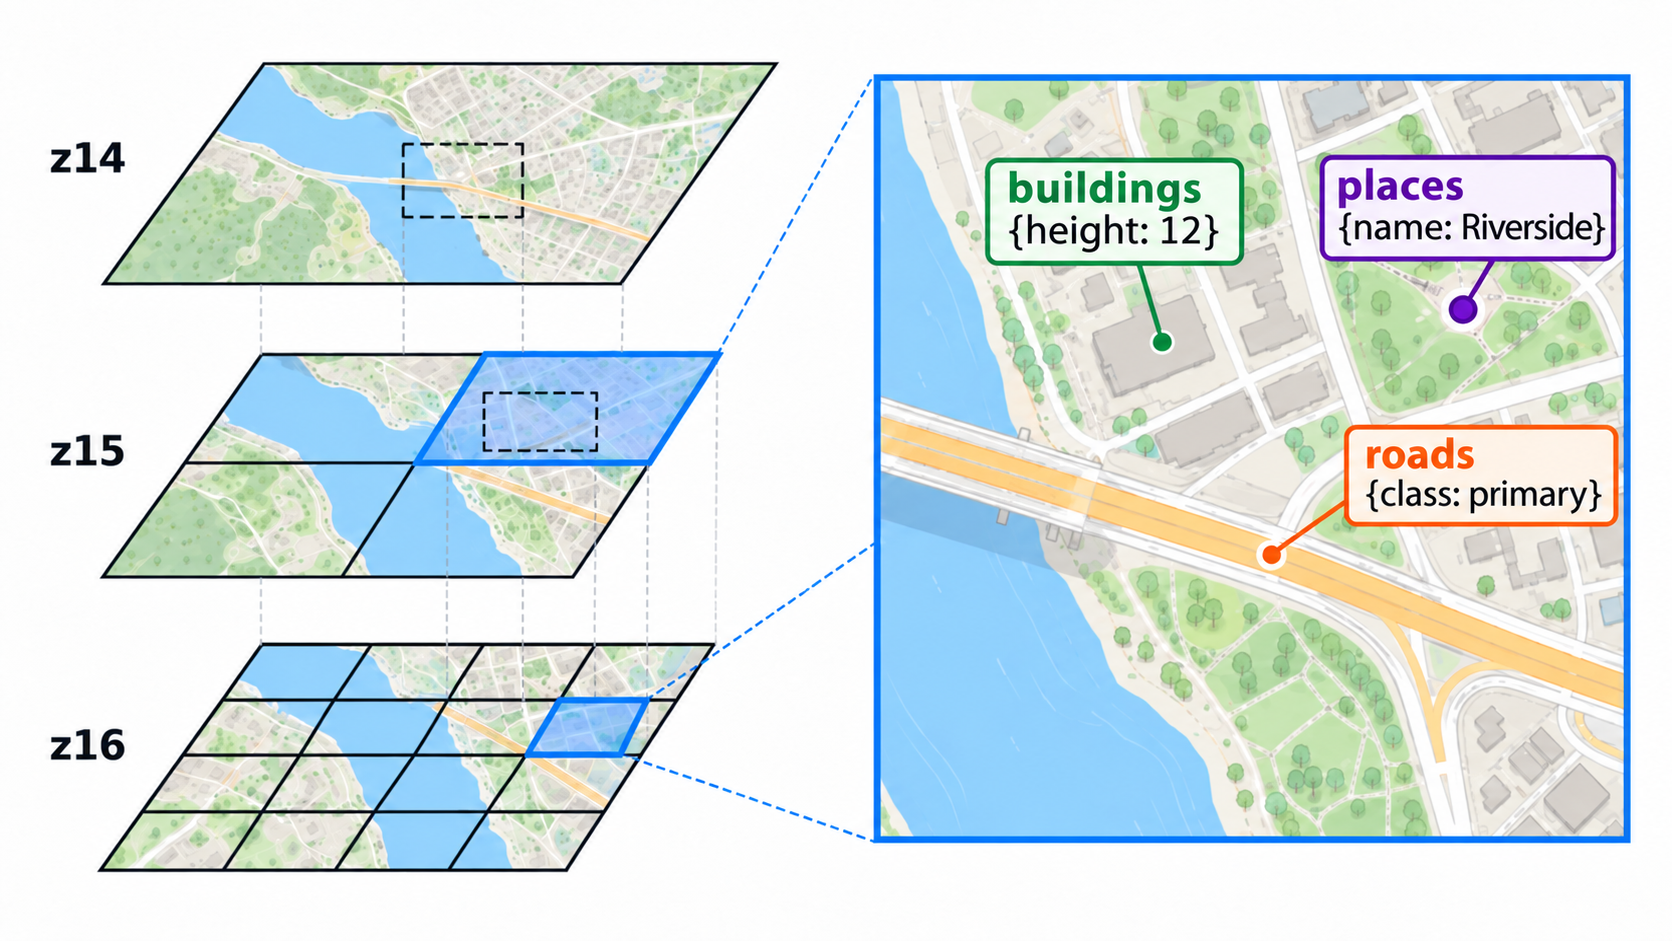
\includegraphics[width=\columnwidth]{figures/tile_concept_overview.png}
    \caption{A tile pyramid, parent and child tiles, a viewport, and the layers,
    coordinates, features and attributes stored in one tile.}
    \label{fig:tile-concept-overview}
\end{figure}

Each zoom level is generated for its own scale. At low zoom levels only major features
are kept and their shapes are simplified, while deeper levels add smaller features and
finer detail (Figure~\ref{fig:pyramid-generalization}). A tile is therefore a summary of
its area at one scale rather than the union of its four children. Production tile
generators also bound the size of each tile: Tippecanoe, for example, by default limits
a tile to 500~kB of compressed data and 200{,}000 features, lowers the resolution of
tiles that exceed the size limit, and offers options to drop or coalesce features
\citep{tippecanoe}.

\begin{figure}[!tbp]
    \centering
    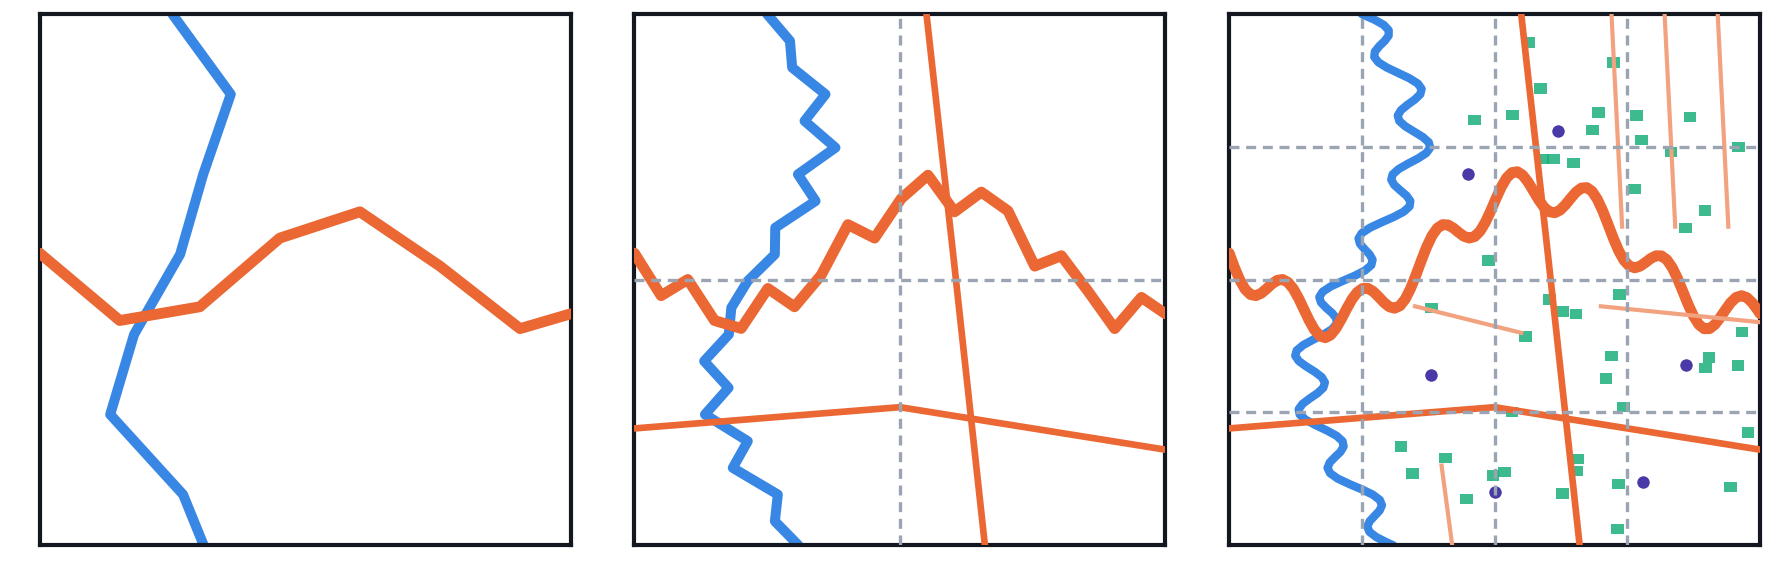
\includegraphics[width=\columnwidth]{figures/pyramid_generalization.png}
    \caption{The same area at three zoom levels: features and detail are added as
    zoom increases.}
    \label{fig:pyramid-generalization}
\end{figure}

Inside a tile, geometry is stored as integer coordinates on a local grid, the
\emph{extent}, conventionally 4096$\times$4096 units \citep{mapbox_mvt_spec_2_1}.
The tile does not record its own position: its $z/x/y$ address is kept outside the tile,
and the tile format itself does not prescribe a pyramid \citep{mapbox_mvt_spec_2_1,
maplibre_mlt_overview}. Every tile is encoded independently, so an encoder can exploit
repetition only among the features of one tile, and each tile repeats its own layer,
column or stream structure.

We distinguish four quantities that are easily conflated. \emph{Spatial tile
granularity} is the geographic area and corresponding content grouped into one
independently encoded tile at a given logical level of detail. \emph{Coordinate extent}
is the integer grid used to represent coordinates inside that tile. \emph{Encoded tile
size} is the resulting number of bytes. \emph{Rendered tile size} is the screen-space
size used by a client. Increasing coordinate extent alone changes precision, not spatial
granularity; in our experiment it is increased together with spatial aggregation so that
the coarser encoding unit retains approximately the same coordinate precision.

% ------------------------------------------------------------
\subsection{Overzoom, metatiles and sparse pyramids}
\label{sec:bg-overzoom}

The dense quadtree pyramid is the default, but practitioners already depart from it,
mainly to reduce the number of stored tiles and requests.

\paragraph{Overzoom.} A client may display a tile at zoom levels deeper than the deepest
level stored, scaling the tile up instead of requesting its children. The extent is the
main limit on this practice: the extent field of MVT is an unsigned 32-bit integer whose
value 4096 is a default rather than a maximum \citep{mapbox_mvt_spec_2_1}, and MLT
declares the extent per layer and notes that a larger extent gives more precision at the
cost of more bytes \citep{maplibre_mlt_overview}. Developer proposals build on this.
A MapLibre proposal argued that ``using a large tile extent allows you to tile your
dataset only as far as is necessary'' \citep{maplibre_gljs_2507}; a Planetiler feature
request asks for an extent of 16384 at the maximum zoom so that a small tileset can be
overzoomed, instead of raising the maximum zoom, which would greatly increase the archive
size \citep{planetiler_1286}; and Tippecanoe can add extra detail at the maximum zoom to
improve precision when overzooming \citep{tippecanoe}. On the client side, MapLibre GL JS
now splits a deep-overzoomed source tile into virtual child tiles in a worker and
overscales only the last few levels, by default four \citep{maplibre_gljs_mapoptions}.

\paragraph{Metatiles.} Raster tile servers commonly render and store \emph{metatiles},
usually blocks of $8\times8$ tiles, because rendering one large area is cheaper than
rendering many small ones, labels are placed more consistently, and fewer files need to
be stored \citep{osm_wiki_metatiles}. Metatiles are a server-side unit, however: clients
still request and receive individual tiles.

\paragraph{Larger tiles.} Vector tile services have also offered larger tiles directly.
The Tilezen service (formerly Mapzen) served 256- and 512-pixel tiles, stating that
a single 512-pixel request is equivalent to four 256-pixel requests, and listed fewer
requests, better label placement, smaller files and less disk space for offline use
among the advantages of the larger size \citep{tilezen_service}. The 512-pixel vector
tile has since become the convention of WebGL renderers such as MapLibre GL JS
\citep{maplibre_gljs_vectorsource}.

\paragraph{Sparse pyramids.} Tippecanoe can generate a variable-depth pyramid that omits
child tiles wherever the parent is detailed enough to be overzoomed \citep{tippecanoe}.
A corresponding Planetiler proposal asks for variable tile depth so that descendants
need not be generated where an ancestor already represents the required detail
\citep{planetiler_1574}. Archives such as PMTiles can store such sparse pyramids, but
clients need a way to distinguish a tile that is intentionally missing, and should be
replaced by an overzoomed ancestor, from one that is empty. A design proposal for
MapLibre adds this distinction to tiled sources and TileJSON
\citep{maplibre_stylespec_1869}.

\paragraph{The rendered tile.} These approaches increase how much information a stored
tile carries, but not the size of the unit that the client renders: MapLibre GL JS, for
example, requires vector sources to use a tile size of 512 pixels
\citep{maplibre_gljs_vectorsource}. Their motivations are primarily rendering precision,
storage and request count. They do not provide a controlled measurement of compression
as a function of the spatial boundary of one independently encoded unit. The denser
variants studied here apply a related idea at every logical zoom: a tile covers the area
of multiple conventional cells while a larger coordinate extent preserves approximately
the same spatial precision.

% ------------------------------------------------------------
\subsection{Feature-oriented and column-oriented tile encodings}
\label{sec:bg-encodings}

The Mapbox Vector Tile (MVT) format encodes a tile as a Protocol Buffers message with
named layers. Each layer holds a sequence of feature records; a record contains the
feature's geometry, written as integer drawing commands with zigzag-encoded coordinate
deltas, and its attributes, written as indices into tables of keys and values shared by
the layer \citep{mapbox_mvt_spec_2_1}. The layout is thus feature-oriented
(Figure~\ref{fig:mvt-mlt-streams}a), and redundancy across features is exploited mainly
through the shared key and value tables and, in practice, by gzip applied to the whole
tile.

MapLibre Tiles (MLT) organizes vector-tile content by column
\citep{tremmel2025mlt, maplibre_mlt_v1}. Within a layer, each property of all features,
such as geometry type, vertex offsets, vertex coordinates or an attribute, is stored as
a column, and each column is split into \emph{streams} of same-typed values, for example
presence, data, length and offset streams. Every stream carries its own metadata,
namely the number of values, the byte length and the encoding
\citep{maplibre_mlt_overview}. Streams are compressed with lightweight encodings such as
dictionary, run-length and delta encoding combined with integer packing, chosen per
stream by the encoder (Figure~\ref{fig:mvt-mlt-streams}b). The original evaluation reports
compression up to three times better than MVT over whole tilesets and more than six
times better for some large tiles \citep{tremmel2025mlt}. MapLibre's public benchmarks on
two planet-scale basemaps report smaller gains after gzip: the stable MLT~v1 reduces
gzipped archive size by about 15\% for OpenMapTiles and 5\% for Protomaps, and the
experimental MLT~v2 by about 18\% and 10\% \citep{maplibre_mlt_benchmarks}.
The same benchmarks show that disabling a dictionary shared by several columns enlarges
the uncompressed archive by about 25\% for one of the two basemaps \citep{maplibre_mlt_benchmarks},
an indication of how much the format depends on redundancy that exists within one tile.
Unlike MVT's per-feature property types, MLT declares one type per property column
within a layer of a tile; mixed input types therefore require normalization during
conversion \citep{maplibre_mlt_mvt_compat}.


The pinned Rust implementation also supports experimental MLT v2. It retains the
columnar layer model while changing stream/schema metadata, interleaved integer RLE
and FastPFOR block layout, and supporting bit-packed dictionary codes. Additional
v2 codecs exist but are disabled in this experiment. We compare versions with the
same common settings as a robustness test, not as a codec-option benchmark
\citep{maplibre_mlt_rust_pinned}.

% Figure: feature-oriented (MVT) vs column-oriented (MLT) layout of one layer,
% and the effect of encoding-unit size on fixed per-stream metadata.
% Requires: \usepackage{tikz}
\begin{figure*}[t]
\centering
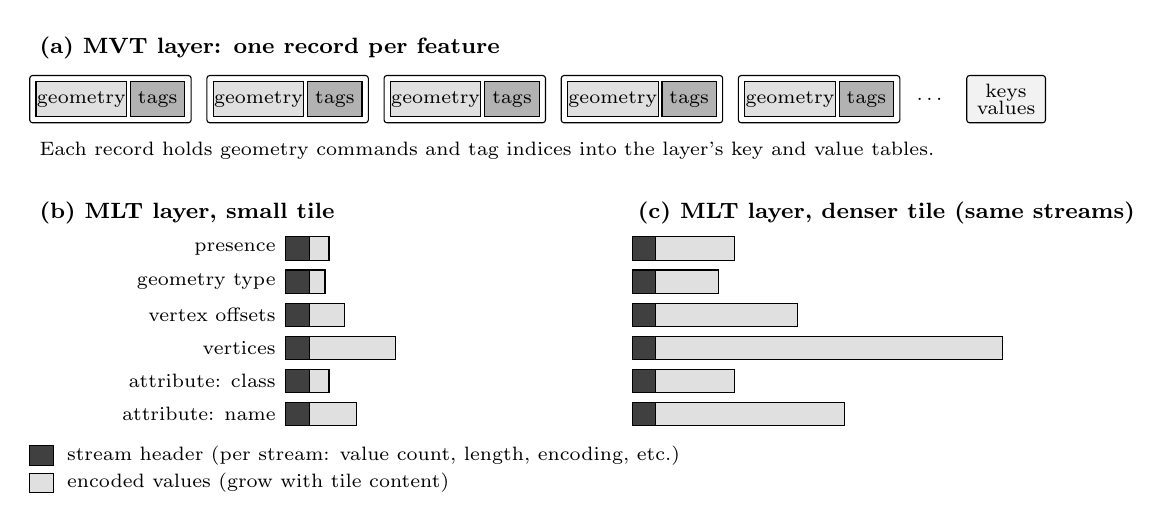
\begin{tikzpicture}[x=1cm, y=1cm, font=\scriptsize,
    hdr/.style={draw, fill=black!75, minimum height=0.32cm, inner sep=0pt},
    pay/.style={draw, fill=black!12},
    rec/.style={draw, rounded corners=1pt},
    lbl/.style={anchor=east, inner sep=2pt}]

  % ---------------- (a) MVT ----------------
  \node[anchor=west, font=\footnotesize\bfseries] at (-2.6,3.55)
        {(a) MVT layer: one record per feature};
  \foreach \i in {0,...,4} {
    \pgfmathsetmacro{\x}{-2.6+\i*2.25}
    \draw[rec] (\x,2.6) rectangle ++(2.05,0.6);
    \draw[pay] (\x+0.08,2.68) rectangle ++(1.15,0.44);
    \node at (\x+0.655,2.9) {geometry};
    \draw[draw, fill=black!30] (\x+1.28,2.68) rectangle ++(0.69,0.44);
    \node at (\x+1.625,2.9) {tags};
  }
  \node at (8.85,2.9) {\dots};
  \draw[rec, fill=black!5] (9.3,2.6) rectangle ++(1.0,0.6);
  \node[align=center] at (9.8,2.9) {keys\\[-2pt]values};
  \node[anchor=west] at (-2.6,2.25)
        {Each record holds geometry commands and tag indices into the layer's key and value tables.};

  % ---------------- (b) MLT, small tile ----------------
  \node[anchor=west, font=\footnotesize\bfseries] at (-2.6,1.45)
        {(b) MLT layer, small tile};
  \node[anchor=west, font=\footnotesize\bfseries] at (5.0,1.45)
        {(c) MLT layer, denser tile (same streams)};

  \def\names{{"presence","geometry type","vertex offsets","vertices","attribute: class","attribute: name"}}
  \def\small{{0.25,0.20,0.45,1.10,0.25,0.60}}
  \foreach \k in {0,...,5} {
    \pgfmathsetmacro{\y}{1.0-\k*0.42}
    \pgfmathparse{\names[\k]}\edef\nm{\pgfmathresult}
    \pgfmathsetmacro{\w}{\small[\k]}
    \pgfmathsetmacro{\W}{min(4*\small[\k],4.6)}
    % small tile
    \node[lbl] at (0.6,\y) {\nm};
    \draw[fill=black!75] (0.65,\y-0.15) rectangle ++(0.3,0.30);
    \draw[pay] (0.95,\y-0.15) rectangle ++(\w,0.30);
    % dense tile
    \draw[fill=black!75] (5.05,\y-0.15) rectangle ++(0.3,0.30);
    \draw[pay] (5.35,\y-0.15) rectangle ++(\W,0.30);
  }

  % legend
  \draw[fill=black!75] (-2.6,-1.75) rectangle ++(0.3,0.25);
  \node[anchor=west] at (-2.25,-1.625) {stream header (per stream: value count, length, encoding, etc.)};
  \draw[pay] (-2.6,-2.1) rectangle ++(0.3,0.25);
  \node[anchor=west] at (-2.25,-1.975) {encoded values (grow with tile content)};
\end{tikzpicture}
\caption{Feature-oriented and column-oriented layouts of one tile layer.
(a)~MVT stores a sequence of feature records.
(b)~MLT stores each property of all features as a column, split into streams of same-typed values;
every stream carries a header.
(c)~When a spatial encoding unit holds more content, streams become longer, amortizing per-stream
headers and exposing longer value sequences to lightweight encodings. MLT also contains layer- and
column-level structural bytes not drawn here; Section~\ref{sec:results-streams} reports total
non-payload structural share separately from stream-header share. Proportions are schematic.}
\label{fig:mvt-mlt-streams}
\end{figure*}

% ------------------------------------------------------------
\subsection{Encoding granularity in columnar storage and block compression}
\label{sec:bg-granularity}

The dependence of compression on the amount of data in one encoding unit is well known
outside cartography. Column stores compress data well because values of one column are
stored together and lightweight encodings can be applied to long runs of similar values
\citep{abadi2006compression}, and empirical studies of Parquet and ORC show that the
choice and effectiveness of encodings depend on the data within each unit
\citep{zeng2023columnar, kuschewski2023btrblocks}. These formats expose the unit size as a
parameter. Parquet lets the writer choose the size of row groups and data pages; its
documentation notes that larger pages carry less header overhead and recommends row
groups of 512~MB to 1~GB \citep{parquet_configurations}. ORC divides files into stripes of
typically about 200~MB and compresses streams in chunks of 256~kB by default, noting that
larger chunks compress better at the cost of memory \citep{orc_spec_v1}. Spatial Parquet
carries these ideas over to geospatial data lakes \citep{saeedan2022spatialparquet}.

General-purpose compressors show the same dependence. DEFLATE, the algorithm behind gzip,
finds repetitions within a sliding window of 32~kB \citep{rfc1951, rfc1952}, so data that
repeat across separately compressed files cannot be exploited. The Zstandard
documentation describes this as the small-data problem: the smaller the input, the
harder it is to compress, because at the start of a new input there is no past to build
upon, and it offers trained dictionaries, whose gains are concentrated in the first few
kilobytes, as a remedy \citep{zstd_readme}.

A vector tile differs from these settings in two ways. Its encoding unit is small,
typically kilobytes rather than megabytes (Appendix~\ref{app:traffic}), and its spatial
granularity is not a free parameter of the encoder: it follows from the tile matrix and
the generalization policy. Coordinate extent can be configured independently, but it
controls the local coordinate grid rather than the geographic area of the encoded unit.

% ------------------------------------------------------------
\subsection{Related work}
\label{sec:bg-related}

Prior work approaches this question from several adjacent directions. The original MLT
evaluation compares MLT and MVT on existing tiles and reports especially large gains for
some large tiles \citep{tremmel2025mlt}. MapLibre's current planet-scale benchmarks go
further and explicitly show that naturally large tiles benefit more from MLT
\citep{maplibre_mlt_benchmarks}. These are important precedents, but tile size is an
observed property of the corpus: the spatial boundary of the independently encoded tile
is not manipulated.

Other studies manipulate quantities that are related to granularity but confound it
with another change. GeoTile reports compressed vector-tile sizes across zoom levels,
where spatial footprint changes together with feature selection and level of detail
\citep{li2018geotile}. Feathered Tiles studies adaptive spatial partitioning and targets
roughly uniform tile payloads, but does not measure a compression-versus-partition-size
curve \citep{dufilie2014feathered}. HiFIVE systematically reduces byte size by pruning
records, attributes and values within a fixed tile, so its intervention is content
reduction rather than a change of the spatial encoding unit
\citep{bahadori2026hifive}. Variable-depth pyramids and overzooming in Tippecanoe and
Planetiler change which pyramid levels are stored, not the compression boundary at a
fixed logical zoom \citep{tippecanoe, planetiler_1574, planetiler_1286}.

These distinctions matter because changing zoom, fidelity, pyramid depth or observed
payload size does not isolate spatial granularity. To our knowledge, no prior work has
systematically varied the area represented by each independently encoded vector tile
under approximately matched-content and matched-LoD conditions and quantified the
resulting raw and externally compressed size, particularly for column-oriented MLT
relative to feature-oriented MVT. Studies of columnar storage
\citep{abadi2006compression, zeng2023columnar, kuschewski2023btrblocks,
saeedan2022spatialparquet} establish the general importance of encoding-unit size, but
at much larger, non-cartographic block sizes.

% ============================================================
% Data and Methods — draft v2
% Citation keys resolve against references.bib (v. 2026-10-16d).
% Requires: natbib, booktabs, tabularx, tikz, amsmath, graphicx.
% Variant names are macros so that they can be renamed in one place.
%
% OPEN ITEMS FOR THIS SECTION (each is also marked TODO at its place):
%  [M1] PDOK: the study area was clipped manually. Add a bounds check to the analyzer,
%       record the clip bounds in the normalization manifest, then fill in the area
%       (Table tab:datasets-structure) and add PDOK to the study-area paragraph.
%  [M2] DONE: source and normalized statistics are generated from results.sqlite;
%       Table tab:datasets-normalized includes measured GPKG feature/vertex counts.
%       Raw PDOK GML vertex counts remain unavailable (not used in these tables).
%  [M3] Dataset provenance: data dates of BGT and NWI, swisstopo product name and nominal
%       scale; add one citation per dataset to the DATASETS section of references.bib.
%  [M4] Attributes: confirm that all attributes were kept for PDOK, USFWS, swisstopo and
%       OSM (only Natural Earth is reduced to a field subset in profile_rules.yaml).
%  [M5] DONE: Standard MVT samples for all maps are generated by manage.py maps;
%       zoom labels and explanatory text are typeset in LaTeX.
%  [M6] Check the qualitative dataset characterizations against tile-level statistics.
%  [M7] DONE: both formats are recompressed at gzip level 6, mtime=0 for analysis;
%       stored lengths are retained and compared in gzip_check.
%  [M8] DONE (from output_analysis_core.py): ratio of sums; deduplicated tiles counted
%       per address; headline gzip sizes use deterministic recompression.
%  [M9] Not for the paper: in the OSM profile, layer "buildings" holds all points,
%       lines, polygons and other relations, "transportation" holds route relations.
%       Describe OSM layers by content in Results; consider renaming in the profile.
%  [M10] Before publishing code: remove the inactive netherlands_amsterdam profile and the
%       copied PDOK prefixes in the OSM profile; move PeakMemory/get_output_size out of
%       the legacy .planetiler module imported by gdal_tiles.py.
% ============================================================

\providecommand{\VStd}{Standard}
\providecommand{\VDfour}{Dense-4}
\providecommand{\VDsixteen}{Dense-16}

\section{Data and Methods}
\label{sec:method}

The experiment converts five heterogeneous vector datasets into tile pyramids in five
variants, encodes every variant in MVT, MLT v1 and MLT v2, and compares the paired
encodings tile by tile. Preparation is
split into two stages: Stage~A normalizes each raw source once into a canonical
GeoPackage, and Stage~B generates all tile variants from that GeoPackage, so that the
variants of one dataset differ only in tiling parameters.

% ------------------------------------------------------------
\subsection{Datasets}
\label{sec:data}

The corpus was chosen to cover different ways in which geospatial data are produced,
because the production process largely determines how much geometry and how many
attributes a map carries per unit area. It contains a generalized small-scale reference
map (Natural Earth), a national large-scale topographic register (PDOK), two thematic
survey products (USFWS wetlands and the swisstopo geological map) and a crowdsourced
dataset (OpenStreetMap). Table~\ref{tab:datasets-provenance} lists their provenance and
Figure~\ref{fig:datasets} shows samples.

Processing whole national or global datasets at three granularities exceeded the memory
and time available for the GDAL-based pipeline, so each dataset was clipped to a study
area (Table~\ref{tab:datasets-structure}). The areas were chosen to contain dense content
for each dataset: the eastern United States for Natural Earth, the Säntis region of
north-eastern Switzerland for the swisstopo map, and the same $0.4^\circ\times0.4^\circ$
area around New Orleans for both USFWS and OSM. The last choice gives a matched pair: two
datasets with very different content over identical geography, which helps to separate
the effect of content from that of location.
% TODO [M1]: add the PDOK study area here once its clip bounds are recorded
%            (PDOK was clipped manually, outside the profile).


\begin{table*}[!tp]
\centering
\caption{Provenance and characteristics of the five datasets.}
\label{tab:datasets-provenance}
\small
\begin{tabularx}{\textwidth}{
    @{}l
    >{\raggedright\arraybackslash}p{3.0cm}
    >{\raggedright\arraybackslash}X
    >{\raggedright\arraybackslash}p{2.1cm}
    >{\raggedright\arraybackslash}p{2.1cm}
    @{}
}
\toprule
Dataset &
Producer &
Content and production mode &
Nominal scale &
Data date \\
\midrule

Natural Earth &
NACIS &
Global physical and cultural reference layers;
generalized cartography at three scales &
1:10m--1:110m &
2021-12 \\

\addlinespace

PDOK BGT &
Dutch public authorities via PDOK &
Large-scale topographic base register
(buildings, roads, land cover, street furniture);
authoritative, continuously updated data &
1:500--1:5{,}000 &
2026-07
(snapshot, approx.) \\

\addlinespace

USFWS wetlands &
U.S.\ Fish and Wildlife Service (NWI) &
Wetland and deepwater habitat polygons for
Louisiana; Cowardin classification;
photo-interpreted thematic mapping &
1:24{,}000 &
2026-05
(release) \\

\addlinespace

swisstopo geology &
Federal Office of Topography swisstopo &
Structural Map of the Helvetic Zone,
Geological Special Map No.~128;
stratigraphic units, folds and tectonic
structures; compiled geological mapping &
1:100{,}000 &
2011
(vector edition) \\

\addlinespace

OSM Louisiana &
OpenStreetMap contributors &
Buildings, transport, land use and points
of interest for Louisiana;
crowdsourced geographic data &
Variable &
2026-09-12 \\

\bottomrule
\end{tabularx}

\vspace{2pt}
\begin{minipage}{\textwidth}
\footnotesize
\textit{Note.}
Dates refer to the dataset version or acquisition snapshot
used in the experiments, not necessarily to the dates of
original field surveys or imagery.
PDOK BGT is continuously updated; its snapshot month
is approximate.
The USFWS date denotes the May 2026 NWI release.
The swisstopo date denotes the 2011 vector edition
of Geological Special Map No.~128 (original map: 2010).
Map scales describe source cartography rather than
the zoom levels of the generated vector tiles.
\end{minipage}
\end{table*}

\begin{table*}[!tp]
\centering
\caption{Raw sources and study areas. Size, source layers, features and fields refer
to the whole raw source; fields are distinct attribute columns summed over layers (for
OSM, tag keys exposed by the GDAL OSM driver). Tile layers and the logical zoom range
refer to the tiled study area. Areas are geodesic areas of declared clipping bounds;
an em dash denotes missing bounds (PDOK). Small extent overruns for USFWS and
swisstopo are recorded in the analysis checks.}
\label{tab:datasets-structure}
\small
\setlength{\tabcolsep}{4pt}
\begin{tabular}{@{}l r r r r r r c@{}}
\toprule
 & \multicolumn{4}{c}{Raw source} & \multicolumn{3}{c}{Study area} \\
\cmidrule(lr){2-5}\cmidrule(l){6-8}
Dataset & MB & Layers & Features & Fields & km$^2$ & Tile layers & Zoom \\
\midrule
% Generated by analysis.extended_report from hash-verified inventories and extended tiles.
Natural Earth & 446 & 183 & 350{,}371 & 12{,}762 & 4.4\,M & 5 & 4--11 \\
PDOK BGT & 53 & 26 & 190{,}294 & 379 & --- & 10 & 3--14 \\
USFWS & 1{,}328 & 4 & 657{,}058 & 21 & 1{,}719 & 1 & 3--14 \\
swisstopo & 46 & 4 & 16{,}319 & 47 & 737 & 1 & 3--14 \\
OSM & 146 & 5 & 1{,}863{,}746 & 3{,}300 & 1{,}719 & 2 & 4--14 \\
\bottomrule

\end{tabular}
% Data rows: analysis.paper_tables, results.sqlite. TODO [M1]: PDOK bounds.
\end{table*}

\begin{table*}[!tp]
\centering
\caption{Measured structure of the normalized GeoPackages used for tile generation.
Size is the on-disk GeoPackage size in MiB; features, vertices and attribute fields
are summed over its layers.}
\label{tab:datasets-normalized}
\small
\begin{tabular}{@{}l r r r r r@{}}
\toprule
Dataset & MiB & Layers & Features & Vertices & Fields \\
\midrule
% Generated by analysis.extended_report from hash-verified inventories and extended tiles.
Natural Earth & 86.5 & 183 & 60{,}574 & 3{,}401{,}476 & 11{,}048 \\
PDOK BGT & 222.3 & 26 & 190{,}294 & 8{,}915{,}989 & 379 \\
USFWS & 108.6 & 4 & 41{,}781 & 5{,}840{,}438 & 21 \\
swisstopo & 0.8 & 1 & 213 & 34{,}560 & 10 \\
OSM & 14.9 & 5 & 15{,}621 & 722{,}903 & 584 \\
\bottomrule

\end{tabular}
\end{table*}

The datasets differ along the dimensions that matter for a columnar encoder.
Natural Earth has few features per unit area but many layers and attributes.
USFWS consists almost entirely of one polygon layer with very detailed boundaries,
about 210 vertices per feature in the raw source, and few attributes. PDOK is dense in
features of many classes with rich attribute schemas. The swisstopo map has few features
over a small area. OSM combines dense buildings with sparser lines and points and a very
large, sparse tag vocabulary.
% TODO [M6]: check these characterizations against tile-level statistics.

Figure~\ref{fig:datasets} shows three nested views per dataset from the \VStd{}
MVT archives. The stored zoom levels and tile addresses were selected for each map's
characteristic content and fixed in a reproducible region configuration. Square
viewports lie inside both the selected tile and the dataset bounds at that zoom;
clipped margins outside those bounds are excluded. Magenta outlines mark the next
view, while zoom labels and palette explanations are typeset in LaTeX. OSM and USFWS
use the same viewports for a direct comparison of coastal Louisiana. Complete tile
addresses, viewport bounds, approximate ground sizes and color inventories are
exported with the figures.

% Generated by python manage.py maps; text stays in LaTeX.
\begin{figure*}[p]
\centering
\begingroup
\setlength{\tabcolsep}{2pt}
\renewcommand{\arraystretch}{1}
\begin{tabular}{@{}cccc@{}}
\begin{minipage}[t]{0.205\textwidth}\vspace{0pt}\centering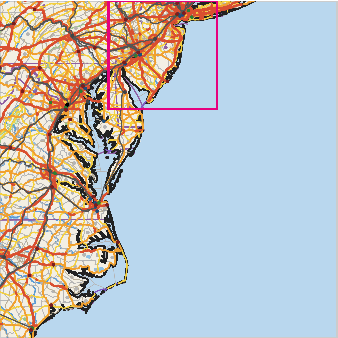
\includegraphics[width=\linewidth]{figures/map_natural_earth_vector_z5.pdf}\par\vspace{1pt}\scriptsize $z=5$\end{minipage} & \begin{minipage}[t]{0.205\textwidth}\vspace{0pt}\centering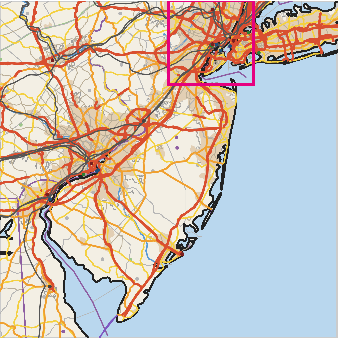
\includegraphics[width=\linewidth]{figures/map_natural_earth_vector_z7.pdf}\par\vspace{1pt}\scriptsize $z=7$\end{minipage} & \begin{minipage}[t]{0.205\textwidth}\vspace{0pt}\centering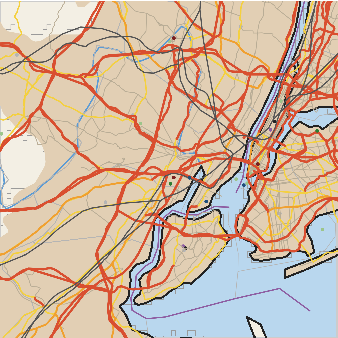
\includegraphics[width=\linewidth]{figures/map_natural_earth_vector_z9.pdf}\par\vspace{1pt}\scriptsize $z=9$\end{minipage} & \begin{minipage}[t]{0.34\textwidth}\vspace{1pt}\footnotesize\raggedright \textbf{(a) Natural Earth}\\ New York / New Jersey.\par\smallskip Colors are illustrative: blue water, pale land, tan urban areas, green parks, red/orange/yellow roads, purple state boundaries and gray county boundaries. Points mark places and transport facilities. Source: Natural Earth / NACIS.\end{minipage} \\[5pt]
\begin{minipage}[t]{0.205\textwidth}\vspace{0pt}\centering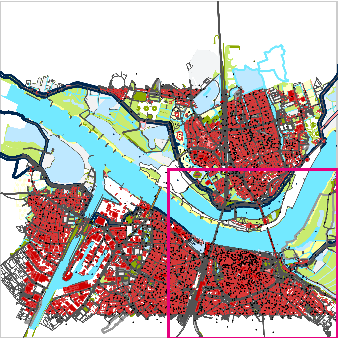
\includegraphics[width=\linewidth]{figures/map_pdok_netherlands_infrostructure_z12.pdf}\par\vspace{1pt}\scriptsize $z=12$\end{minipage} & \begin{minipage}[t]{0.205\textwidth}\vspace{0pt}\centering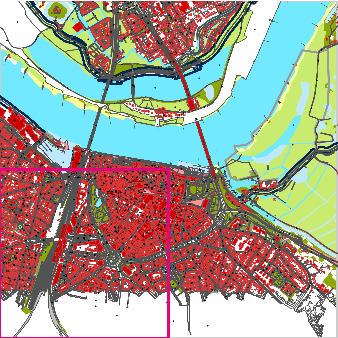
\includegraphics[width=\linewidth]{figures/map_pdok_netherlands_infrostructure_z13.pdf}\par\vspace{1pt}\scriptsize $z=13$\end{minipage} & \begin{minipage}[t]{0.205\textwidth}\vspace{0pt}\centering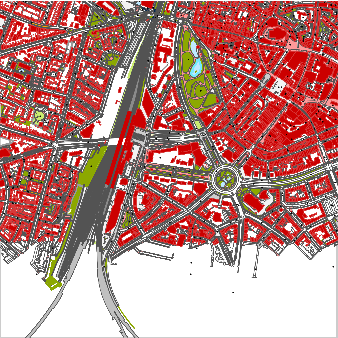
\includegraphics[width=\linewidth]{figures/map_pdok_netherlands_infrostructure_z14.pdf}\par\vspace{1pt}\scriptsize $z=14$\end{minipage} & \begin{minipage}[t]{0.34\textwidth}\vspace{1pt}\footnotesize\raggedright \textbf{(b) PDOK BGT}\\ Nijmegen, Netherlands.\par\smallskip The palette follows the BGT standard visualization: red buildings, blue water, green vegetation and white local roads/paved areas; gray denotes classes without an assigned standard color. Source: PDOK.\end{minipage} \\[5pt]
\begin{minipage}[t]{0.205\textwidth}\vspace{0pt}\centering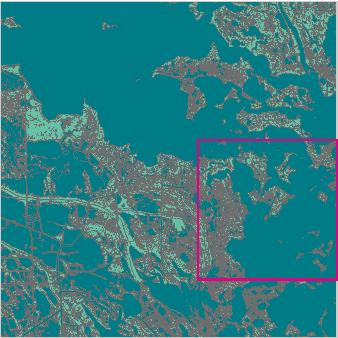
\includegraphics[width=\linewidth]{figures/map_usfws_luisiana_wetlands_geopackage_z10.pdf}\par\vspace{1pt}\scriptsize $z=10$\end{minipage} & \begin{minipage}[t]{0.205\textwidth}\vspace{0pt}\centering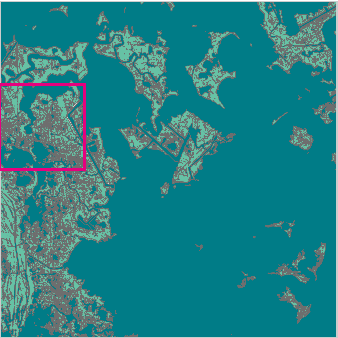
\includegraphics[width=\linewidth]{figures/map_usfws_luisiana_wetlands_geopackage_z12.pdf}\par\vspace{1pt}\scriptsize $z=12$\end{minipage} & \begin{minipage}[t]{0.205\textwidth}\vspace{0pt}\centering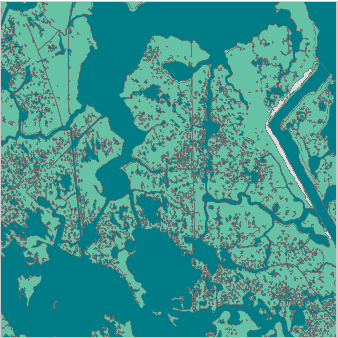
\includegraphics[width=\linewidth]{figures/map_usfws_luisiana_wetlands_geopackage_z14.pdf}\par\vspace{1pt}\scriptsize $z=14$\end{minipage} & \begin{minipage}[t]{0.34\textwidth}\vspace{1pt}\footnotesize\raggedright \textbf{(c) USFWS wetlands}\\ coastal Louisiana.\par\smallskip The NWI palette distinguishes forested/shrub wetlands (dark green), emergent wetlands (light green), tidal wetlands (teal), and water classes (blue); unclassified polygons are light gray. Source: U.S. Fish and Wildlife Service, National Wetlands Inventory.\end{minipage} \\[5pt]
\begin{minipage}[t]{0.205\textwidth}\vspace{0pt}\centering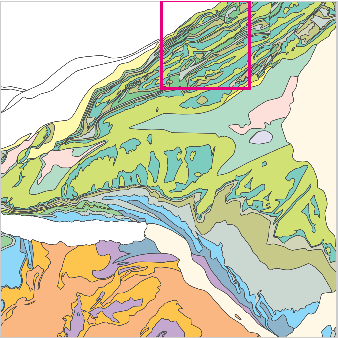
\includegraphics[width=\linewidth]{figures/map_swisstopo_mountains_vector_z10.pdf}\par\vspace{1pt}\scriptsize $z=10$\end{minipage} & \begin{minipage}[t]{0.205\textwidth}\vspace{0pt}\centering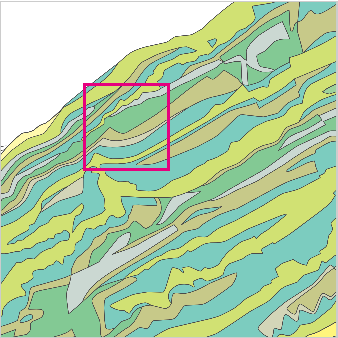
\includegraphics[width=\linewidth]{figures/map_swisstopo_mountains_vector_z12.pdf}\par\vspace{1pt}\scriptsize $z=12$\end{minipage} & \begin{minipage}[t]{0.205\textwidth}\vspace{0pt}\centering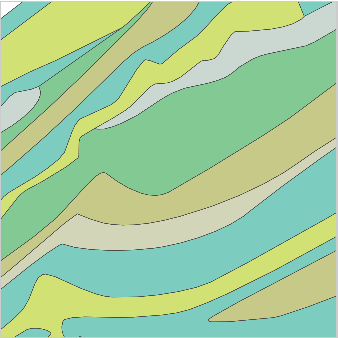
\includegraphics[width=\linewidth]{figures/map_swisstopo_mountains_vector_z14.pdf}\par\vspace{1pt}\scriptsize $z=14$\end{minipage} & \begin{minipage}[t]{0.34\textwidth}\vspace{1pt}\footnotesize\raggedright \textbf{(d) swisstopo geology}\\ Saentis, Switzerland.\par\smallskip Colors distinguish geological units using the swisstopo legend and the retained \texttt{SYMBOL}/\texttt{INDEX\_} attributes. White denotes units without an assigned legend color. Source: swisstopo, Structural Map of the Helvetic Zone, sheet 128.\end{minipage} \\[5pt]
\begin{minipage}[t]{0.205\textwidth}\vspace{0pt}\centering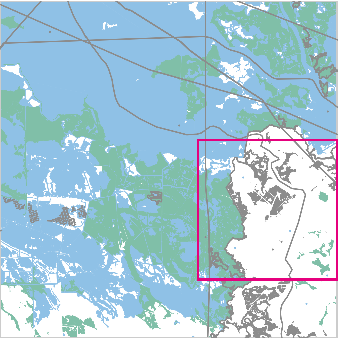
\includegraphics[width=\linewidth]{figures/map_louisiana-260912_z10.pdf}\par\vspace{1pt}\scriptsize $z=10$\end{minipage} & \begin{minipage}[t]{0.205\textwidth}\vspace{0pt}\centering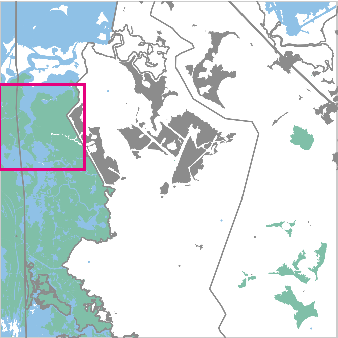
\includegraphics[width=\linewidth]{figures/map_louisiana-260912_z12.pdf}\par\vspace{1pt}\scriptsize $z=12$\end{minipage} & \begin{minipage}[t]{0.205\textwidth}\vspace{0pt}\centering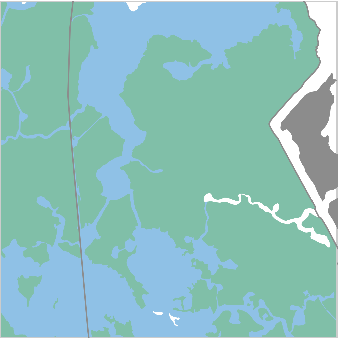
\includegraphics[width=\linewidth]{figures/map_louisiana-260912_z14.pdf}\par\vspace{1pt}\scriptsize $z=14$\end{minipage} & \begin{minipage}[t]{0.34\textwidth}\vspace{1pt}\footnotesize\raggedright \textbf{(e) OpenStreetMap}\\ coastal Louisiana.\par\smallskip An illustrative tag-based palette shows water in blue, wetlands in teal, vegetation in green, buildings in brown, roads/routes in orange and other objects in gray. Classification uses retained OSM tags rather than merged tile-layer names. Source: \copyright{} OpenStreetMap contributors, ODbL.\end{minipage} \\[5pt]
\end{tabular}
\endgroup
\caption{The five datasets at three zoom levels, rendered from Standard MVT tiles. Views are nested from left to right; magenta outlines locate the next view. Square viewports stay within the configured data bounds at each zoom. USFWS and OSM show the same coastal Louisiana areas.}
\label{fig:datasets}
\label{fig:map-natural_earth_vector}
\label{fig:map-pdok_netherlands_infrostructure}
\label{fig:map-usfws_luisiana_wetlands_geopackage}
\label{fig:map-swisstopo_mountains_vector}
\label{fig:map-louisiana-260912}
\end{figure*}



% ------------------------------------------------------------
\subsection{Normalization}
\label{sec:normalization}

Each raw source was converted with GDAL into a canonical GeoPackage in Web Mercator
(EPSG:3857) with two-dimensional geometries, clipped once to the study area and indexed
spatially. Source layers were mapped onto a common set of semantic kinds (water, land,
boundary, transport, place, building, infrastructure, terrain) so that all datasets can
be rendered with one style sheet and inspected visually. Several source layers can be
merged into one tile layer, which gives between one (USFWS) and ten (PDOK) tile layers per
dataset (Table~\ref{tab:datasets-structure}). For Natural Earth, which has 183 source
layers with heterogeneous schemas, only a common subset of attributes (feature class,
names in four languages, administrative codes and rank fields) was kept. Geometry is not
altered by this mapping.
% TODO [M4]: confirm that all attributes were kept for the other four datasets.
% NOTE [M9]: OSM layer names do not match their content (see header).
A manifest records the source and rule hashes, CRS, bounds, layer counts, feature
identity strategy and GDAL version, so that every normalized layer can be traced back to
its source.

The grouping of source layers into tile layers affects the absolute size of both
encodings, and of MLT in particular, because it determines how many features share one
set of streams. The mapping rules are identical for all variants of a dataset and for
both encodings. However, changing tile granularity can change which property types
co-occur within an output layer, so the resulting type conversions are measured
separately (Section~\ref{sec:encoding}).

% ------------------------------------------------------------

\subsection{Tile generation and source identity}\label{sec:tile-generation}
MVT is regenerated with GDAL 3.13.3 from the same normalized sources and study
regions. Globally unique feature IDs equal original GeoPackage FIDs plus disjoint
source-layer offsets. A separate SQLite table maps these IDs to original layers and
FIDs. A derived GeoPackage materializes only this FID remapping; exhaustive SQL
comparison verifies that every geometry BLOB and attribute cell equals the source.
GDAL's \texttt{-preserve\_fid} writes the IDs into MVT; no provenance attribute is
added. IDs identify normalized records, including distinct records in different layers
that describe the same real-world object. Historical archives are stored separately.

Standard and Dense retain the original layer grouping and generation rules:
simplification is 1.6 tile units below the maximum zoom and 1.0 at maximum zoom;
buffer width is 80 units per 4096 extent units. Extent scales with linear cell width,
preserving the intended ground-coordinate resolution at matched logical zoom.
Tile-size and feature limits are $2^{31}-1$. GDAL writes MBTiles and directly repacks
MVT payloads into PMTiles~\citep{gdal_mvt,pmtiles_v3}.

\subsection{Five variants and three comparisons}\label{sec:granularity}
Standard uses extent 4096. Aggregated-4 and Aggregated-16 regroup $2\times2$ and
$4\times4$ Standard cells into one unit, translating coordinates by integer multiples
of 4096. They retain the exact feature multiset: geometry command sequences, precision,
fragments, duplicates, ID presence, attributes and typed protobuf values. MVT keys and
values are interned across children, giving MVT the enlarged dictionary scope too.
No feature is merged, deduplicated, simplified or regenerated. An independent parse
of every serialized aggregate must reproduce the translated typed multiset.
Dense instead regenerates the larger cell, changing clipping, buffering and possibly
representation. Figure~\ref{fig:variants} illustrates the Dense spatial arrangement;
Aggregated uses the same parent layout while retaining internal Standard fragments.

\begin{table}[!tbp]\centering\small
\caption{Five variants. Offset $d$ relates stored zoom $z$ to logical zoom
$\ell=z+d$. Factor denotes geographic area relative to a Standard cell.}
\label{tab:variants}\setlength{\tabcolsep}{3pt}
\begin{tabular}{@{}lrrrl@{}}\toprule
Variant & Factor & Extent & $d$ & Content\\
\midrule% Generated by analysis.extended_report from measured extended results; do not edit.
Standard & 1 & 4096 & 0 & Conventional baseline \\
Aggregated-4 & 4 & 8192 & 1 & Exact Standard multiset \\
Aggregated-16 & 16 & 16384 & 2 & Exact Standard multiset \\
Dense-4 & 4 & 8192 & 1 & Regenerated \\
Dense-16 & 16 & 16384 & 2 & Regenerated \\
\bottomrule
\end{tabular}\end{table}
% Figure: Standard pyramid vs. Dense-4 / Dense-16 stored tiles.
% Requires: \usepackage{tikz}; variant-name macros \VStd, \VDfour, \VDsixteen.
\begin{figure}[t]
\centering
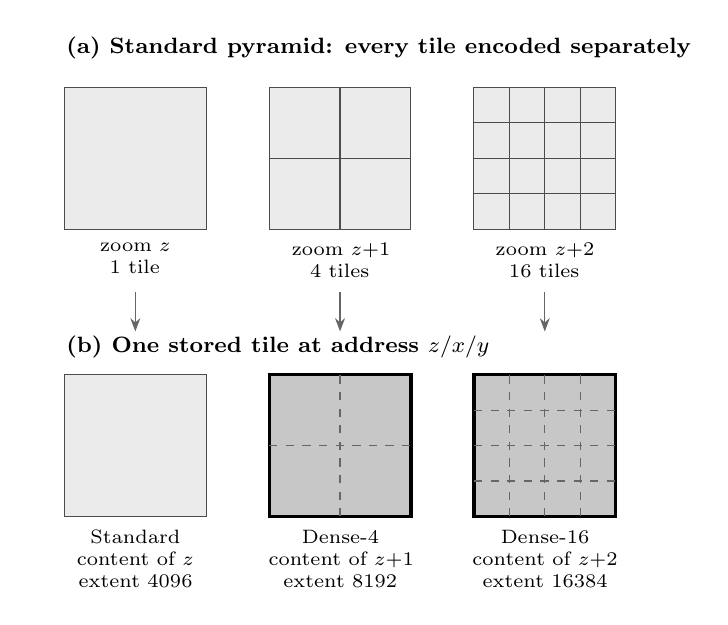
\begin{tikzpicture}[x=1cm, y=1cm, font=\scriptsize,
    unit/.style={draw=black!70, fill=black!8},
    dense/.style={draw=black, very thick, fill=black!22},
    lab/.style={align=center, text width=2.5cm, anchor=north}]
  \def\S{1.8}
  % ---- (a) Standard pyramid: separately encoded tiles ----
  \node[anchor=west, font=\footnotesize\bfseries] at (-0.1,2.55)
    {(a) \VStd{} pyramid: every tile encoded separately};
  \foreach \n/\x/\lbl in {1/0/{zoom $z$\\1 tile}, 2/2.6/{zoom $z{+}1$\\4 tiles}, 4/5.2/{zoom $z{+}2$\\16 tiles}} {
    \pgfmathsetmacro{\c}{\S/\n}
    \foreach \i in {1,...,\n} \foreach \j in {1,...,\n}
      \draw[unit] ({\x+(\i-1)*\c},{(\j-1)*\c+0.25}) rectangle ++(\c,\c);
    \node[lab] at (\x+\S/2,0.2) {\lbl};
  }
  % ---- (b) stored tile at z/x/y ----
  \node[anchor=west, font=\footnotesize\bfseries] at (-0.1,-1.25)
    {(b) One stored tile at address $z/x/y$};
  \draw[unit] (0,-3.4) rectangle ++(\S,\S);
  \node[lab] at (\S/2,-3.45) {\VStd\\content of $z$\\extent 4096};
  \draw[dense] (2.6,-3.4) rectangle ++(\S,\S);
  \draw[dashed, black!60] (2.6+\S/2,-3.4) -- ++(0,\S) (2.6,-3.4+\S/2) -- ++(\S,0);
  \node[lab] at (2.6+\S/2,-3.45) {\VDfour\\content of $z{+}1$\\extent 8192};
  \draw[dense] (5.2,-3.4) rectangle ++(\S,\S);
  \foreach \k in {1,2,3} {
    \draw[dashed, black!60] (5.2+\k*\S/4,-3.4) -- ++(0,\S);
    \draw[dashed, black!60] (5.2,-3.4+\k*\S/4) -- ++(\S,0);
  }
  \node[lab] at (5.2+\S/2,-3.45) {\VDsixteen\\content of $z{+}2$\\extent 16384};
  % arrows from (a) to (b)
  \foreach \x in {0,2.6,5.2}
    \draw[-{Stealth}, black!60] (\x+\S/2,-0.55) -- (\x+\S/2,-1.05);
\end{tikzpicture}
\caption{Spatial-granularity variants. (a)~In the \VStd{} pyramid an area at
logical zoom $z+1$ or $z+2$ is partitioned into 4 or 16 independently encoded tiles.
(b)~The \VDfour{} and \VDsixteen{} variants generate one independently encoded tile
over the corresponding parent area using the feature-selection and simplification rules
of logical zoom $z+1$ or $z+2$. Coordinate extent grows with the linear spatial factor
to preserve approximately the same ground-coordinate precision; extent is not itself
the granularity variable. Aggregated-4 and Aggregated-16 use these same larger
footprints and extents, but translate and retain the complete Standard feature
multiset instead of regenerating it. Dashed lines mark the internal Standard
boundaries; their existing fragments and buffered copies remain in Aggregated.}
\label{fig:variants}
\end{figure}


At each logical zoom, comparisons match parent-cell coordinates over the geographic
intersection of available Standard groups, Aggregated and Dense blocks. Missing
edge blocks are reported separately. Standard--Aggregated measures the
\emph{compression-unit effect}; Aggregated--Dense measures the
\emph{tile-regeneration effect}; Standard--Dense measures the total effect.
The regeneration effect is not attributed exclusively to clipping.

\subsection{Pinned Rust encoding and validation}\label{sec:encoding}
Both versions use the official \texttt{mlt-core 0.22.1} source shipped with
\texttt{maplibre-tiles 0.4.1}~\citep{maplibre_tiles_py,maplibre_mlt_rust_pinned}.
A framed CLI adapter calls Rust directly; Python handles archive I/O. Source SHA-256,
Cargo lockfile, Rust version, binary and adapter hashes, and settings accompany each
conversion. Both versions use Native/4G with tessellation and sorting disabled,
FSST, FastPFOR and shared dictionaries enabled. Fixed v2 defaults enable packed
dictionary codes and disable ALP, float dictionaries, second-order delta and rANS
vertices. We do not search codec options.

Every encoded layer is decoded and compared to the Rust MVT importer's layer using
the official CLI verification rules. Those rules permit integer-width changes,
polygon winding normalization and absent/null equivalence. The importer can unify
mixed property types, including string coercion; per-property source types and
imported column types are exported. Thus the round trip checks consistency after
import, not strict equality to every typed MVT value. Source/imported feature and
vertex counts expose additional normalization. Aggregation uses its own stronger
typed-protobuf multiset check before MLT encoding.
Exact equivalence is established at the MVT input boundary. Since column-type
unification depends on the values sharing a unit, Aggregated MLT can normalize
types differently from Standard MLT. The measured fixed-input byte effect includes
this format constraint; it does not isolate compression mechanics from normalization.

Earlier historical validation failed at 48 addresses under an internal 20 MiB Rust
guard: 22 Natural Earth, 25 PDOK and one USFWS. The stock 64 MiB guard in 0.4.1
still rejected 17 of those addresses. The extended CLI passes 256 MiB explicitly
to MVT import, MLT parsing, decoding and the read-only structural walker. This guard
is distinct from Docker's quota and does not bound total RSS. The largest new
PDOK Dense-16 input exposed a separate 32 MiB protobuf element-memory guard;
raising only the MLT decoder budget did not affect that earlier import stage.
Budget-only patches expose explicit limits through both readers and the walker;
their original defaults and encoding algorithms remain unchanged.
After writing, every physical PMTiles archive is read back. Its addresses, raw
lengths and payload hashes must match the measurements, linking native validation
to the actual stored MLT bytes and detecting missing or changed payloads.

\subsection{Measurements and additive decomposition}\label{sec:metrics}
Raw bytes and independently recompressed gzip bytes (level 6, timestamp zero) are
measured per address. Unique stored payloads and complete archive sizes are recorded
separately. MLT saving within one variant is
\begin{equation}\label{eq:saving}
S=100\left(1-\frac{\sum B_{\rm MLT}}{\sum B_{\rm MVT}}\right).
\end{equation}
For one format and compression state over identical matched blocks, let $B_S$,
$B_A$ and $B_D$ denote Standard, Aggregated and Dense bytes. Then
\begin{equation}\label{eq:decomposition}
\underbrace{B_S-B_D}_{\text{total}}=
\underbrace{B_S-B_A}_{\text{aggregation}}+
\underbrace{B_A-B_D}_{\text{regeneration}}.
\end{equation}
Component percentages all divide by $B_S$ and remain additive. They are distinct
from MLT-versus-MVT percentage-point gains.

Content counts include feature instances, unique provenance IDs at each logical
zoom, explicit stored vertices and MoveTo components. Components include line parts,
rings and points; they are not necessarily clipping fragments. Repeated instances
share an ID. Repeated vertices share ID and integer coordinates within a comparison
block; implicit polygon closures are excluded. These are observable redundancy
measures, not a causal partition into clipping and buffering. Identities are not
deduplicated across logical zooms.

The official version-aware annotated walker partitions each MLT frame into metadata
and encoded data regions. For frame bytes $F$ and stream payload bytes $P$,
\begin{equation}\label{eq:structural-share}R_{\rm struct}=(F-P)/F.\end{equation}
Stream length counts expanded logical values after integer RLE in both versions;
vertices count coordinate pairs, booleans logical positions. Values/stream and
payload bytes/value mix different stream roles. Structural statistics count each
unique MVT payload input once, while transfer sizes count addresses; they do not
provide an exact algebraic attribution of transfer savings to particular codecs.

\section{Results}\label{sec:results}
% Generated by analysis.extended_report from measured extended results; do not edit.
\providecommand{\ExtOneRawAggregationMin}{2.4}
\providecommand{\ExtOneRawAggregationMax}{55.4}
\providecommand{\ExtOneRawRegenerationMin}{-6.1}
\providecommand{\ExtOneRawRegenerationMax}{24.2}
\providecommand{\ExtOneRawTotalMin}{-1.7}
\providecommand{\ExtOneRawTotalMax}{79.6}
\providecommand{\ExtOneRawAggregationPositive}{5}
\providecommand{\ExtOneGzipAggregationMin}{3.3}
\providecommand{\ExtOneGzipAggregationMax}{65.4}
\providecommand{\ExtOneGzipRegenerationMin}{-6.6}
\providecommand{\ExtOneGzipRegenerationMax}{7.0}
\providecommand{\ExtOneGzipTotalMin}{-2.2}
\providecommand{\ExtOneGzipTotalMax}{72.5}
\providecommand{\ExtOneGzipAggregationPositive}{5}
\providecommand{\ExtTwoRawAggregationMin}{2.2}
\providecommand{\ExtTwoRawAggregationMax}{52.8}
\providecommand{\ExtTwoRawRegenerationMin}{-6.2}
\providecommand{\ExtTwoRawRegenerationMax}{23.7}
\providecommand{\ExtTwoRawTotalMin}{-2.5}
\providecommand{\ExtTwoRawTotalMax}{76.5}
\providecommand{\ExtTwoRawAggregationPositive}{5}
\providecommand{\ExtTwoGzipAggregationMin}{3.7}
\providecommand{\ExtTwoGzipAggregationMax}{66.4}
\providecommand{\ExtTwoGzipRegenerationMin}{-6.7}
\providecommand{\ExtTwoGzipRegenerationMax}{5.9}
\providecommand{\ExtTwoGzipTotalMin}{-2.3}
\providecommand{\ExtTwoGzipTotalMax}{72.4}
\providecommand{\ExtTwoGzipAggregationPositive}{5}
\providecommand{\ExtTiles}{45{,}689}
\providecommand{\ExtCheckedAddresses}{91{,}378}
\providecommand{\ExtRoundtripDifferences}{0}
\providecommand{\ExtAggregateBlocks}{9{,}042}

\subsection{Fixed-content aggregation}\label{sec:results-granularity}
All \ExtAggregateBlocks{} aggregate blocks pass the typed feature-multiset check.
The expanded corpus contains \ExtTiles{} MVT addresses, each also encoded as MLT
v1 and v2. Table~\ref{tab:main} reports MLT saving relative to its own MVT input.
For $4\times4$ controlled aggregation, raw v1 byte reductions range from
\ExtOneRawAggregationMin\% to \ExtOneRawAggregationMax\%, positive in
\ExtOneRawAggregationPositive{} datasets; v2 ranges from \ExtTwoRawAggregationMin\%
to \ExtTwoRawAggregationMax\%, positive in \ExtTwoRawAggregationPositive{} datasets.
After gzip the ranges are \ExtOneGzipAggregationMin--\ExtOneGzipAggregationMax\%
and \ExtTwoGzipAggregationMin--\ExtTwoGzipAggregationMax\%. All buffered and clipped
Standard instances are retained in these comparisons.

\begin{table*}[!tp]\centering\small
\caption{MLT savings relative to MVT (\%) within each variant, using byte sums
over addresses. A4/A16 are Aggregated; D4/D16 are Dense.}\label{tab:main}
\begin{tabular}{@{}llrrrrr@{}}\toprule
Dataset & Variant & Tiles & Raw v1 & Raw v2 & Gzip v1 & Gzip v2\\
\midrule% Generated by analysis.extended_report from measured extended results; do not edit.
Natural Earth & Std & 25{,}800 & 34.4 & 52.3 & 10.8 & 14.3 \\
 & A4 & 6{,}554 & 52.8 & 64.9 & 12.4 & 15.9 \\
 & A16 & 1{,}705 & 61.0 & 69.9 & 14.5 & 20.3 \\
 & D4 & 6{,}554 & 38.0 & 52.1 & 14.7 & 17.6 \\
 & D16 & 1{,}705 & 44.5 & 53.4 & 20.0 & 22.9 \\
PDOK BGT & Std & 153 & 62.4 & 63.9 & 28.4 & 29.8 \\
 & A4 & 68 & 62.7 & 64.2 & 29.0 & 30.7 \\
 & A16 & 37 & 63.0 & 64.5 & 29.4 & 31.1 \\
 & D4 & 70 & 62.4 & 64.0 & 29.0 & 30.5 \\
 & D16 & 39 & 62.7 & 64.1 & 29.3 & 30.9 \\
USFWS & Std & 606 & 45.0 & 46.1 & 14.9 & 16.0 \\
 & A4 & 184 & 45.6 & 46.4 & 15.2 & 16.4 \\
 & A16 & 71 & 46.1 & 46.8 & 15.6 & 16.8 \\
 & D4 & 190 & 46.4 & 47.1 & 15.5 & 16.6 \\
 & D16 & 81 & 47.4 & 48.0 & 16.2 & 17.3 \\
swisstopo & Std & 435 & 19.7 & 29.5 & 12.8 & 10.8 \\
 & A4 & 128 & 29.4 & 35.2 & 17.0 & 16.2 \\
 & A16 & 47 & 34.5 & 37.7 & 19.0 & 19.2 \\
 & D4 & 130 & 26.6 & 32.7 & 16.1 & 15.3 \\
 & D16 & 50 & 30.3 & 33.8 & 17.8 & 17.8 \\
OSM & Std & 576 & 46.9 & 53.7 & 13.1 & 17.6 \\
 & A4 & 178 & 48.7 & 54.8 & 14.0 & 19.3 \\
 & A16 & 70 & 49.7 & 55.6 & 14.7 & 20.4 \\
 & D4 & 182 & 49.6 & 55.4 & 14.9 & 20.0 \\
 & D16 & 76 & 50.6 & 56.2 & 16.0 & 21.2 \\
\bottomrule
\end{tabular}\end{table*}
% Generated from docs/data/extended/results.sqlite by analysis.extended_report.
\begin{figure*}[!tp]
\centering
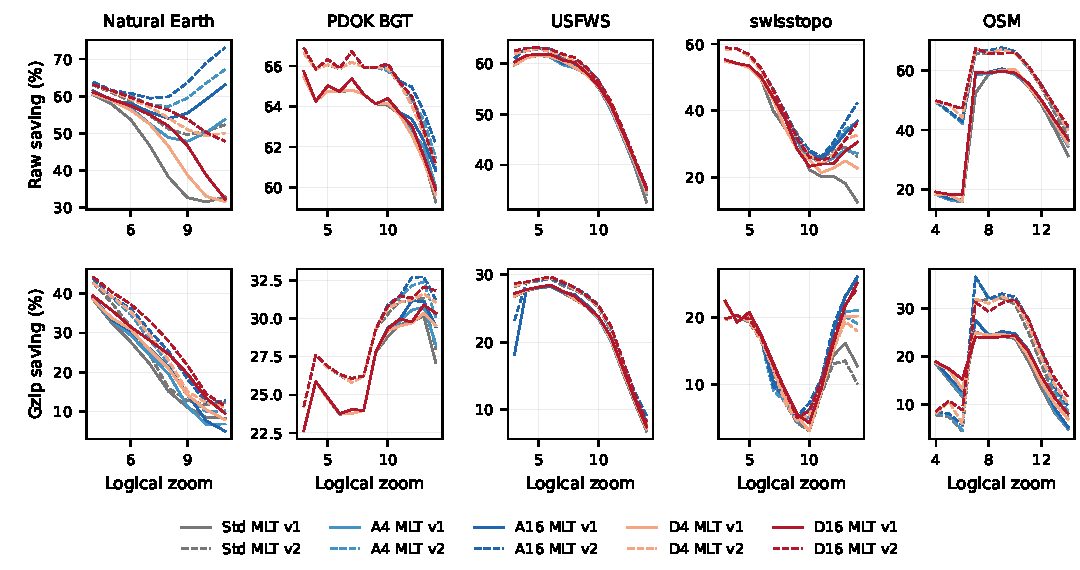
\includegraphics[width=\textwidth]{figures/analysis_zoom_aligned.pdf}
\caption{MLT saving relative to each variant's MVT input by logical zoom,
raw (top) and after independent gzip-6 (bottom). Colours distinguish Standard,
Aggregated-4/16 and Dense-4/16; solid curves are v1 and dashed curves v2.
The additive decomposition separately matches geographic parent blocks.}
\label{fig:zoom-aligned}
\end{figure*}


\subsection{Additional regeneration effects}\label{sec:results-density}
Table~\ref{tab:decomposition} separates aggregation from regeneration. Both components
divide by matched Standard bytes, so they sum to the total reduction. Negative
regeneration values mean that Dense requires more bytes than the exact aggregate.
For $4\times4$ blocks the total gzip reduction ranges from
\ExtOneGzipTotalMin\% to \ExtOneGzipTotalMax\% for v1 and
\ExtTwoGzipTotalMin\% to \ExtTwoGzipTotalMax\% for v2.

\begin{table*}[!tp]\centering\footnotesize
\caption{Additive reductions relative to matched Standard bytes (\%). A: aggregation;
R: regeneration; T: total. Integer bytes and per-zoom values are exported separately;
rounding can change the displayed component sum by 0.1 percentage points.}
\label{tab:decomposition}
\begin{tabular}{@{}lrlrrrrrr@{}}\toprule
& & & \multicolumn{3}{c}{MLT v1} & \multicolumn{3}{c}{MLT v2}\\
Dataset & Factor & State & A & R & T & A & R & T\\
\midrule% Generated by analysis.extended_report from measured extended results; do not edit.
Natural Earth & 4 & raw & 42.1 & 19.4 & 61.5 & 41.0 & 18.1 & 59.1 \\
 & 4 & gzip & 50.7 & 5.0 & 55.8 & 50.8 & 4.8 & 55.5 \\
 & 16 & raw & 55.4 & 24.2 & 79.6 & 52.8 & 23.7 & 76.5 \\
 & 16 & gzip & 65.4 & 7.0 & 72.5 & 66.4 & 5.9 & 72.4 \\
PDOK BGT & 4 & raw & 2.0 & 0.1 & 2.1 & 1.8 & 0.2 & 1.9 \\
 & 4 & gzip & 2.5 & -0.6 & 2.0 & 3.0 & -0.8 & 2.2 \\
 & 16 & raw & 2.4 & 0.9 & 3.3 & 2.2 & 0.8 & 3.0 \\
 & 16 & gzip & 3.3 & -0.2 & 3.0 & 3.7 & -0.4 & 3.3 \\
USFWS & 4 & raw & 3.2 & -2.4 & 0.8 & 2.7 & -2.5 & 0.2 \\
 & 4 & gzip & 2.9 & -2.7 & 0.2 & 3.1 & -2.9 & 0.2 \\
 & 16 & raw & 4.4 & -6.1 & -1.7 & 3.7 & -6.2 & -2.5 \\
 & 16 & gzip & 4.3 & -6.6 & -2.2 & 4.4 & -6.7 & -2.3 \\
swisstopo & 4 & raw & 31.2 & 2.5 & 33.7 & 28.1 & 2.6 & 30.7 \\
 & 4 & gzip & 25.9 & 2.6 & 28.5 & 26.8 & 2.6 & 29.4 \\
 & 16 & raw & 42.1 & 4.2 & 46.3 & 37.3 & 4.5 & 41.7 \\
 & 16 & gzip & 34.4 & 4.5 & 38.9 & 36.0 & 4.3 & 40.3 \\
OSM & 4 & raw & 7.5 & -1.6 & 5.8 & 6.4 & -2.0 & 4.4 \\
 & 4 & gzip & 6.1 & -1.3 & 4.8 & 7.0 & -1.6 & 5.5 \\
 & 16 & raw & 10.2 & -5.6 & 4.5 & 8.9 & -6.0 & 2.9 \\
 & 16 & gzip & 8.3 & -4.4 & 3.9 & 9.6 & -4.8 & 4.8 \\
\bottomrule
\end{tabular}\end{table*}

Standard and Aggregated feature and vertex totals are exactly equal over matched
blocks; Dense need not preserve them (Table~\ref{tab:content-differences}). Components
include inherent multipart geometry and rings. Repeated coordinates identify
observable ID/coordinate redundancy within a block, without attributing its cause.

\begin{table*}[!tp]\centering\footnotesize
\caption{Matched content counts (thousands). A: Aggregated; D: Dense. Repeated vertices
share ID and coordinates within a block.}\label{tab:content-differences}
\setlength{\tabcolsep}{3pt}
\begin{tabular}{@{}lrrrrrrrrr@{}}\toprule
& & \multicolumn{2}{c}{Instances} & \multicolumn{2}{c}{Vertices} &
\multicolumn{2}{c}{Source IDs$^*$} & \multicolumn{2}{c}{Repeated vertices}\\
Dataset & Factor & A & D & A & D & A & D & A & D\\
\midrule% Generated by analysis.extended_report from measured extended results; do not edit.
Natural Earth & 4 & 1{,}982.7 & 978.3 & 17{,}994.6 & 14{,}127.0 & 473.8 & 473.8 & 435.0 & 30.5 \\
 & 16 & 1{,}982.7 & 683.4 & 17{,}994.6 & 13{,}028.3 & 473.8 & 473.8 & 651.5 & 31.0 \\
PDOK BGT & 4 & 1{,}124.0 & 1{,}101.1 & 10{,}342.3 & 10{,}156.2 & 1{,}079.2 & 1{,}079.2 & 448.3 & 174.7 \\
 & 16 & 1{,}124.0 & 1{,}087.5 & 10{,}342.3 & 10{,}015.8 & 1{,}079.2 & 1{,}079.1 & 531.4 & 173.3 \\
USFWS & 4 & 333.8 & 343.3 & 13{,}807.2 & 13{,}930.4 & 279.5 & 279.4 & 548.1 & 94.2 \\
 & 16 & 333.8 & 361.6 & 13{,}807.2 & 14{,}226.0 & 279.5 & 279.4 & 763.7 & 103.3 \\
swisstopo & 4 & 4.6 & 3.3 & 174.4 & 168.0 & 2.4 & 2.4 & 5.6 & 0.2 \\
 & 16 & 4.6 & 2.8 & 174.4 & 163.3 & 2.4 & 2.4 & 8.2 & 0.2 \\
OSM & 4 & 123.0 & 123.7 & 2{,}048.6 & 2{,}077.7 & 102.2 & 102.2 & 79.0 & 9.1 \\
 & 16 & 123.0 & 127.9 & 2{,}048.6 & 2{,}147.2 & 102.2 & 102.2 & 112.5 & 9.9 \\
\bottomrule
\end{tabular}
\par\smallskip $^*$Unique IDs at each logical zoom, summed across zooms.
\end{table*}

\subsection{Robustness across MLT versions}\label{sec:results-versions}
The paired version comparison holds MVT input and shared encoder settings fixed.
Tables~\ref{tab:main} and~\ref{tab:decomposition} show both the version-specific
relative saving and the controlled aggregation component. Figure~\ref{fig:zoom-aligned}
shows individual logical zooms; absolute totals are dominated by the zooms carrying
most bytes. The decomposition uses common parent blocks, while a coverage export
records unmatched edge support.

\subsection{Stream structure}\label{sec:results-streams}
The native walker accounts for all bytes in every converted MLT tile. Structural
share, expanded logical values per stream and payload bytes per logical value use
consistent definitions in both versions (Table~\ref{tab:streams}). Stream-role
mixtures can change with regeneration; Aggregated provides the stronger control.
These descriptive measurements do not individually establish a causal contribution
to after-gzip savings.

\begin{table*}[!tp]\centering\footnotesize
\caption{Stream structure per unique MVT payload input, using expanded integer-RLE
counts. Structural share is $(F-P)/F$.}\label{tab:streams}
\begin{tabular}{@{}llrrrrrr@{}}\toprule
& & \multicolumn{2}{c}{Values/stream} & \multicolumn{2}{c}{Structure (\%)} & \multicolumn{2}{c}{Payload B/value}\\
Dataset & Variant & v1 & v2 & v1 & v2 & v1 & v2\\
\midrule% Generated by analysis.extended_report from measured extended results; do not edit.
Natural Earth & Std & 34 & 27 & 40.61 & 34.76 & 0.403 & 0.610 \\
 & A4 & 111 & 79 & 22.37 & 17.59 & 0.305 & 0.514 \\
 & A16 & 362 & 249 & 9.03 & 6.83 & 0.273 & 0.472 \\
 & D4 & 47 & 38 & 31.59 & 25.38 & 0.431 & 0.682 \\
 & D16 & 92 & 75 & 18.64 & 13.67 & 0.440 & 0.732 \\
PDOK BGT & Std & 2{,}254 & 3{,}375 & 0.46 & 0.36 & 1.239 & 0.786 \\
 & A4 & 4{,}429 & 6{,}589 & 0.24 & 0.19 & 1.220 & 0.777 \\
 & A16 & 6{,}641 & 9{,}787 & 0.16 & 0.12 & 1.218 & 0.779 \\
 & D4 & 4{,}225 & 6{,}292 & 0.25 & 0.19 & 1.238 & 0.789 \\
 & D16 & 6{,}080 & 9{,}056 & 0.17 & 0.13 & 1.239 & 0.791 \\
USFWS & Std & 668 & 933 & 0.98 & 0.65 & 1.331 & 1.227 \\
 & A4 & 1{,}901 & 2{,}557 & 0.35 & 0.23 & 1.303 & 1.228 \\
 & A16 & 5{,}013 & 6{,}654 & 0.14 & 0.09 & 1.275 & 1.225 \\
 & D4 & 2{,}028 & 2{,}814 & 0.33 & 0.22 & 1.320 & 1.234 \\
 & D16 & 4{,}856 & 6{,}672 & 0.14 & 0.09 & 1.316 & 1.235 \\
swisstopo & Std & 38 & 62 & 10.24 & 8.77 & 2.157 & 1.138 \\
 & A4 & 119 & 145 & 4.81 & 3.89 & 1.597 & 1.154 \\
 & A16 & 313 & 338 & 2.25 & 1.71 & 1.397 & 1.176 \\
 & D4 & 107 & 136 & 5.00 & 4.08 & 1.709 & 1.172 \\
 & D16 & 257 & 292 & 2.48 & 1.92 & 1.512 & 1.204 \\
OSM & Std & 272 & 330 & 2.51 & 1.86 & 1.147 & 0.813 \\
 & A4 & 666 & 770 & 1.15 & 0.81 & 1.052 & 0.786 \\
 & A16 & 1{,}376 & 1{,}550 & 0.61 & 0.42 & 1.010 & 0.770 \\
 & D4 & 683 & 787 & 1.13 & 0.80 & 1.057 & 0.786 \\
 & D16 & 1{,}383 & 1{,}567 & 0.60 & 0.41 & 1.029 & 0.777 \\
\bottomrule
\end{tabular}\end{table*}

\subsection{Gzip and content-normalized size}\label{sec:results-bpv}
Table~\ref{tab:bpv} reports bytes per explicit stored MVT vertex for every format/state
combination. Importer geometry-count diagnostics are supplied separately. Independent
gzip can change the relative MLT advantage, so the after-gzip trend need not match the
raw trend. Table~\ref{tab:bins} separates content-dependent savings by intervention.

\begin{table*}[!tp]\centering\footnotesize
\caption{Bytes per explicit MVT vertex, raw and after deterministic gzip-6.}\label{tab:bpv}
\begin{tabular}{@{}llrrrrrr@{}}\toprule
Dataset & Variant & MVT & MVT+gz & MLT v1 & v1+gz & MLT v2 & v2+gz\\
\midrule% Generated by analysis.extended_report from measured extended results; do not edit.
Natural Earth & Std & 30.21 & 9.51 & 19.81 & 8.48 & 14.42 & 8.15 \\
 & A4 & 24.27 & 4.77 & 11.47 & 4.18 & 8.51 & 4.01 \\
 & A16 & 22.62 & 3.43 & 8.83 & 2.93 & 6.81 & 2.73 \\
 & D4 & 15.68 & 5.60 & 9.72 & 4.78 & 7.52 & 4.61 \\
 & D16 & 10.06 & 4.03 & 5.58 & 3.23 & 4.68 & 3.11 \\
PDOK BGT & Std & 15.59 & 6.50 & 5.87 & 4.66 & 5.62 & 4.57 \\
 & A4 & 15.40 & 6.39 & 5.75 & 4.54 & 5.52 & 4.43 \\
 & A16 & 15.49 & 6.38 & 5.73 & 4.50 & 5.49 & 4.40 \\
 & D4 & 15.57 & 6.54 & 5.85 & 4.65 & 5.61 & 4.55 \\
 & D16 & 15.70 & 6.60 & 5.86 & 4.66 & 5.63 & 4.56 \\
USFWS & Std & 4.38 & 2.65 & 2.41 & 2.26 & 2.36 & 2.23 \\
 & A4 & 4.28 & 2.59 & 2.33 & 2.19 & 2.29 & 2.16 \\
 & A16 & 4.26 & 2.56 & 2.30 & 2.16 & 2.27 & 2.13 \\
 & D4 & 4.41 & 2.65 & 2.37 & 2.24 & 2.33 & 2.21 \\
 & D16 & 4.52 & 2.68 & 2.38 & 2.24 & 2.35 & 2.21 \\
swisstopo & Std & 5.50 & 3.92 & 4.41 & 3.42 & 3.88 & 3.49 \\
 & A4 & 4.30 & 3.05 & 3.04 & 2.53 & 2.79 & 2.56 \\
 & A16 & 3.90 & 2.77 & 2.56 & 2.24 & 2.43 & 2.24 \\
 & D4 & 4.17 & 3.04 & 3.06 & 2.55 & 2.81 & 2.57 \\
 & D16 & 3.68 & 2.73 & 2.57 & 2.25 & 2.44 & 2.25 \\
OSM & Std & 6.24 & 2.91 & 3.31 & 2.53 & 2.88 & 2.39 \\
 & A4 & 5.97 & 2.76 & 3.06 & 2.37 & 2.70 & 2.22 \\
 & A16 & 5.91 & 2.72 & 2.97 & 2.32 & 2.63 & 2.16 \\
 & D4 & 6.10 & 2.79 & 3.07 & 2.37 & 2.72 & 2.23 \\
 & D16 & 6.11 & 2.76 & 3.02 & 2.32 & 2.67 & 2.18 \\
\bottomrule
\end{tabular}\end{table*}

\begin{table*}[!tp]\centering\footnotesize
\caption{Content-dependent MLT savings (\%), pooled separately for Standard,
fixed-content Aggregated and regenerated Dense. Ratios use byte sums; both area
factors are pooled within each extended regime.}\label{tab:bins}
\begin{tabular}{@{}lllrrr@{}}\toprule
Regime & Format & Vertices/tile & Tiles & Raw saving & Gzip saving\\
\midrule% Generated by analysis.extended_report from measured extended results; do not edit.
Aggregated & MLT v1 & $<$100 & 1{,}160 & 11.5 & -9.9 \\
Aggregated & MLT v1 & 100--999 & 848 & 59.0 & 10.1 \\
Aggregated & MLT v1 & 1,000--9,999 & 6{,}204 & 56.7 & 7.3 \\
Aggregated & MLT v1 & 10,000--99,999 & 683 & 54.7 & 16.6 \\
Aggregated & MLT v1 & 100,000$+$ & 147 & 58.5 & 25.5 \\
Aggregated & MLT v2 & $<$100 & 1{,}160 & 24.7 & -1.8 \\
Aggregated & MLT v2 & 100--999 & 848 & 71.9 & 13.7 \\
Aggregated & MLT v2 & 1,000--9,999 & 6{,}204 & 68.6 & 11.6 \\
Aggregated & MLT v2 & 10,000--99,999 & 683 & 61.7 & 20.2 \\
Aggregated & MLT v2 & 100,000$+$ & 147 & 60.1 & 27.5 \\
Dense & MLT v1 & $<$100 & 1{,}374 & -6.3 & -5.1 \\
Dense & MLT v1 & 100--999 & 3{,}183 & 32.1 & 8.6 \\
Dense & MLT v1 & 1,000--9,999 & 3{,}842 & 33.4 & 11.0 \\
Dense & MLT v1 & 10,000--99,999 & 533 & 51.1 & 19.8 \\
Dense & MLT v1 & 100,000$+$ & 145 & 58.3 & 25.8 \\
Dense & MLT v2 & $<$100 & 1{,}374 & 6.6 & 1.1 \\
Dense & MLT v2 & 100--999 & 3{,}183 & 51.2 & 12.0 \\
Dense & MLT v2 & 1,000--9,999 & 3{,}842 & 48.7 & 12.7 \\
Dense & MLT v2 & 10,000--99,999 & 533 & 55.8 & 22.5 \\
Dense & MLT v2 & 100,000$+$ & 145 & 59.8 & 27.6 \\
Standard & MLT v1 & $<$100 & 4{,}528 & -6.8 & -4.0 \\
Standard & MLT v1 & 100--999 & 19{,}732 & 32.7 & 8.6 \\
Standard & MLT v1 & 1,000--9,999 & 2{,}833 & 34.6 & 11.1 \\
Standard & MLT v1 & 10,000--99,999 & 419 & 49.2 & 17.3 \\
Standard & MLT v1 & 100,000$+$ & 58 & 60.8 & 27.7 \\
Standard & MLT v2 & $<$100 & 4{,}528 & 6.4 & 1.4 \\
Standard & MLT v2 & 100--999 & 19{,}732 & 52.2 & 12.4 \\
Standard & MLT v2 & 1,000--9,999 & 2{,}833 & 49.9 & 13.2 \\
Standard & MLT v2 & 10,000--99,999 & 419 & 52.6 & 19.4 \\
Standard & MLT v2 & 100,000$+$ & 58 & 62.3 & 29.3 \\
\bottomrule
\end{tabular}\end{table*}

The native audit compares \ExtCheckedAddresses{} address/format combinations and
records \ExtRoundtripDifferences{} normalized round-trip differences. Attribute
normalization and imported geometry counts remain separate diagnostics; these
checks do not assert strict equality of every original protobuf storage type.

\section{Discussion}\label{sec:discussion}
The exact Aggregated control distinguishes encoding-unit effects from changed map
content. It retains duplicate attributes and fragments from the original boundaries,
while allowing dictionaries and streams to span a larger unit. Its byte reduction
cannot be explained by removing those instances. Dense answers a different practical
question: what happens when a larger cell is generated afresh? Its regeneration
component combines buffering, clipping and representation changes, without attributing
the whole effect to one operation.

Comparing v1 and v2 tests robustness to wire layout and supported encodings under
fixed options. The measured ranges and exceptions are conditional on that build.
Structural share and payload bytes/value describe the outcome, but codec choices and
stream-role mixtures may change together. Five heterogeneous datasets support
descriptive comparisons rather than a universal predictive law.

Gzip already exploits within-unit repetition; its incremental MLT saving can differ
from raw saving. Bytes per vertex controls one content dimension but not attributes,
geometry type, fragments or repeated identities. Exact aggregation provides stronger
control than dividing size by any one count.

Larger units also change retrieval granularity. A client may fetch content beyond
its viewport, invalidate larger cache entries and spend longer decoding one unit.
Fixed-coverage byte accounting does not model an interactive session. Offline archives
and bulk distribution can use smaller totals directly, but choosing a production
tile size requires workload, memory and rendering measurements. Overzoom and
variable-depth pyramids remain different interventions, because they change the
stored pyramid rather than only the encoding boundary at fixed logical zoom.

\section{Threats to Validity}\label{sec:threats}
\paragraph{Content equivalence.}
Only Aggregated preserves the exact typed Standard multiset. Dense must be
interpreted through its regeneration component. Source IDs identify normalized
records, not real-world entities across layers. MoveTo components include rings and
multipart geometry; repeated ID/coordinate occurrences do not isolate clipping from
buffering. Common parent-cell support and a separate coverage export expose the
effect of excluding unmatched boundary blocks.

\paragraph{Semantic normalization.}
Rust can unify property types and normalize geometry during MVT import. Native
round-trip verification checks that representation, allowing winding and integer-width
differences. It does not establish strict protobuf equality, style equivalence or
completeness relative to normalized source data. Type-transition and geometry-count
exports document these qualifications.
The exact Aggregated control applies before MLT import; larger units can introduce
additional mixed-type columns and hence different type normalization. Those transitions
are measured, but are not independently manipulated as a compression mechanism.
New provenance IDs add encoded content, so
historical Python size results are retained separately rather than mixed with the
regenerated primary corpus.

\paragraph{Implementation and memory.}
Both MLT versions use one pinned Rust core and shared settings. MLT v2 remains
experimental and may change. This evaluates granularity, not all possible codec
configurations. The explicit 256 MiB native allocation guard is distinct from process
RSS and Docker's quota; raising a container quota cannot itself alter that internal
guard. The MVT-reader and annotation patches expose budget plumbing without changing encoding.
The official version-aware walker replaces the historical v1-only structural parser.
The historical \texttt{memory limit exceeded} errors were validation failures,
not evidence of absent archive addresses. With the explicit 256 MiB guard the retained-corpus
audit subsequently covered all 36,647 addresses without decoder errors; strict
typed/geometry differences remained a separate diagnostic. These historical
counts are not substituted for validation of the regenerated experiment.

\paragraph{External validity.}
The five fixed study regions and mappings do not establish gains for other schemas,
national coverage or production generalization policies. Address-weighted transfers,
unique payload storage and physical archive size are different measurements. No
session-level overfetch, latency, decoding, rendering or peak-memory benchmark is
inferred from compression totals.
Recorded conversion times are diagnostics of concurrent execution, not controlled
encoding-throughput comparisons.

\section{Conclusion}\label{sec:conclusion}
Fixed-content aggregation separates spatial encoding-unit granularity from tile
regeneration. For $4\times4$ aggregation the raw reduction ranges from
\ExtOneRawAggregationMin\% to \ExtOneRawAggregationMax\% for MLT v1 and
\ExtTwoRawAggregationMin\% to \ExtTwoRawAggregationMax\% for v2. After independent
gzip the ranges are \ExtOneGzipAggregationMin--\ExtOneGzipAggregationMax\% and
\ExtTwoGzipAggregationMin--\ExtTwoGzipAggregationMax\%. The separate regeneration
component shows how practical larger-tile generation modifies that controlled result.
Format comparisons should specify encoding unit, source content, generation policy
and compression state, and distinguish fixed-coverage sizes from interactive delivery.

\section*{Data Availability}\label{sec:data-availability}
The earlier software and statistics releases remain at
\url{https://doi.org/10.5281/zenodo.23459428} and
\url{https://doi.org/10.5281/zenodo.23452598}.
The expanded experiment is supplied in the accompanying repository and its
\texttt{zenodo} software export; local updates do not imply publication of a new
release at those identifiers. Reproduction uses pinned Rust source and lockfile,
source-provenance lookup tables, PMTiles and compressed measurement logs. Observations
are exported as per-tile, per-layer, per-stream and identity Parquet tables, with
SQLite summaries and CSV inputs for the article. Original source licences remain
applicable.

% ============================================================
% Appendix A — Tile sizes in production web maps — draft v1
% Source: real-world-map-traffic.md (measured 2026-10-02).
% OPEN ITEMS:
%  [A1] Yandex Maps serves raster PNG and its own vector tiles; the 3.8 KB median mixes
%       both. Recompute vector-only statistics or drop Yandex from the vector rows.
%  [A2] Keep this appendix to tile sizes; page shares and the Aviasales MLT estimate are
%       deliberately left out (they answer a different question).
% ============================================================

\appendix
\section{Tile sizes in production web maps}
\label{app:traffic}

To see how large the tiles of production web maps are, we recorded the network traffic
of seven web products that show maps: OpenStreetMap, Yandex Maps, Amap, Cian, Airbnb,
Booking.com and Aviasales. Each product was loaded five times in desktop Chrome with a
cold cache and a viewport of $2560\times1600$ CSS pixels at a device pixel ratio of 1.5;
each run opened the map, panned by one map width and one map height and zoomed in once,
waiting for the network to be idle after each step. All requests, including those of web
workers and iframes, were recorded through the DevTools protocol, and tile bodies were
classified by decoding them. On our own archives, the recorded tile sizes matched the
stored sizes exactly (21 of 21 tiles).

Table~\ref{tab:traffic} lists the compressed sizes of individual tiles. The vector tiles
of Amap, Airbnb, Booking.com and Yandex Maps, all in proprietary formats, had medians
between 0.1 and 3.8~KB, and a page view loaded hundreds of them. The only MVT tiles
observed, from Aviasales, were world-level tiles at zoom~3 with a mean of 94~KB.

\begin{table}[!htbp]
\centering
\caption{Compressed size of individual tiles in seven web products (KB, median of runs;
1~KB = 1000 bytes). Measured on 2 October 2026 from one desktop machine.}
\label{tab:traffic}
\footnotesize
\setlength{\tabcolsep}{2.5pt}
\begin{tabular}{@{}l l r r r l@{}}
\toprule
Product & Format & Tiles & Median & P90 & Zoom \\
\midrule
OpenStreetMap & PNG              & 354 & 38.1 & 47.0  & 10, 14 \\
Cian          & PNG              & 363 & 16.3 & 27.5  & 10, 12 \\
Yandex Maps   & PNG + own vector & 677 & 3.8  & 25.9  & 9--11 \\
Amap          & own vector       & 774 & 1.2  & 5.4   & 10 \\
Airbnb        & Google vector    & 269 & 0.1  & 12.6  & 10--13 \\
Booking.com   & Google vector    & 357 & 2.0  & 5.8   & 11--16 \\
Aviasales     & MVT              & 8   & 95.7 & 157.2 & 3 \\
\bottomrule
\end{tabular}

\smallskip
{\scriptsize Tiles: tiles per run; own vector: proprietary vector format.}
% TODO [A1]: vector-only figures for Yandex Maps.
\end{table}

The measurement has clear limits. It used one machine, one network location (Turkey),
one day and first loads only; sites localize by IP address, and street-level zoom was
reached only on OpenStreetMap and Booking.com. The formats of most products are
proprietary, so their sizes indicate the granularity at which vector map data are
delivered, not the size of MVT or MLT tiles with the same content.

\bibliographystyle{abbrvnat}
\raggedright
\bibliography{references}

\end{document}
